% Instituto Nacional de Pesquisas Espaciais - INPE
% carlos.bastarz@inpe.br (15/04/2021)

\documentclass[10pt]{beamer}

% Tema padrão (base)
\usetheme{default}

% Carrega pacotes e macros
% Carregamento dos pacotes utilizados
\usepackage[brazil]{babel}
\usepackage{times}
\usepackage{fontspec}
\usepackage{url}
\usepackage{tikzsymbols}
\usepackage{color}
\usepackage{xcolor}
\usepackage{xcolor-material}
\usepackage{xcolor-solarized}
\usepackage{hanging}
\usepackage{minted}
\usepackage[most]{tcolorbox}
\tcbuselibrary{breakable}
\tcbuselibrary{minted}
\tcbuselibrary{skins}
\usepackage{lipsum}
\usepackage{tabularx}
\usepackage{booktabs}
\usepackage{multicol}
\usepackage{tikz}
\usepackage{verbatim}
\usetikzlibrary{arrows,shapes}
\usepackage{metalogo}
\usepackage{enumerate}
\usepackage{float}
\usepackage{caption}
\usepackage{subcaption}
\usepackage{fontawesome5}
\usepackage{hyperref}
% Macros extras
\definecolor{pretoinpe}{HTML}{515151}
\definecolor{azulinpe}{RGB}{0, 110, 175}
\definecolor{laranjainpe}{RGB}{248, 133, 31}

% Caixas das Dicas (pacote tcolorbox)
% Material Colors
\newtcolorbox{marker}[1][]{enhanced,
  before skip=10mm,after skip=10mm,
  boxrule=1.4pt,left=6mm,right=3mm,top=2mm,bottom=2mm,
  colback=MaterialAmberA100!75,
  colupper=black,
  colframe=pretoinpe,
  underlay={%
    \path[fill=none] (frame.south west) rectangle node[pretoinpe]{\huge\bfseries !} ([xshift=7mm]frame.north west);
    }}
  
% Caixas dos Exemplos (pacote tcolorbox)
% Material Colors
\tcbset{
    texexp/.style={
        colframe=laranjainpe!90,
        colback=white,
        coltitle=black,
        fonttitle=\small\sffamily\bfseries,
        fontupper=\small, 
        fontlower=\small,
        arc=0pt, outer arc=0pt, box align=center, halign=center, valign=center},
        example/.style 2 args={texexp,
        title={\hspace{-4mm}Exemplo \thetcbcounter: #1},label={#2}},
    }
    \newtcblisting{texexp}[1]{texexp,#1}
    \newtcblisting[auto counter,number within=section]{texexptitled}[3][]{%
        example={#2}{#3},#1}
    \newtcolorbox[use counter from=texexptitled]{texexptitledspec}[3][]{%
        example={#2}{#3},#1}

% Caixas dos Exercícios e Soluções (pacote tcolorbox)  
% Material Colors
\NewTColorBox[auto counter,number within=chapter]{exercise}{m+O{}}{%
    enhanced,
    colframe=MaterialGreen900,
    colback=white,
    coltitle=white,
    fonttitle=\bfseries,
    underlay={\begin{tcbclipinterior}
        \shade[inner MaterialGreen900,outer color=white]
            (interior.north west) circle (2cm);
        \draw[help lines,step=5mm,MaterialGreen900,shift={(interior.north west)}]
            (interior.south west) grid (interior.north east);
        \end{tcbclipinterior}},
    title={Exercício~ \thetcbcounter:},
    label={exercise:#1},
    attach title to upper=\quad,
    after upper={\par\hfill\textcolor{white}%
        {\itshape Resposta na página~\pageref{solution:#1}}},
    lowerbox=ignored,
    savelowerto=respostas/exercise-\thetcbcounter.tex,
    record={\string\solution{#1}{respostas/exercise-\thetcbcounter.tex}},
    #2
}

% Esta é a lista de exercícios
\newtcolorbox[auto counter,number within=section,list inside=exam]{texercise}[4][]{%
    texercisestyle,
    listing file={respostas/texercise\thetcbcounter.tex},
    label={exe:#2},
    record={\string\processsol{respostas/texercise\thetcbcounter.tex}{#2}},
    title={Exercício \thetcbcounter\hfill\mdseries Resposta na página \pageref{sol:#2}},
    list text={\vspace{-1em}\hspace{1mm} #3 - resposta na página \pageref{sol:#2}}, #1)}
    
\tcbset{texercisestyle/.style={arc=0.5mm, colframe=MaterialGreen900,
    colback=white, coltitle=white,
    fonttitle=\small\sffamily\bfseries, fontupper=\small, fontlower=\small,
    listing options={style=tcblatex,texcsstyle=*\color{MaterialRed900}},
}}

% \usepackage{hyperref} % for phantomlabel
\newtcbinputlisting{\processsol}[2]{%
    texercisestyle,
    listing only,
    listing file={#1},
    phantomlabel={sol:#2},%
    title={Resposta do Exercício \ref{exe:#2} na página \pageref{exe:#2}},
}

% Caixa dos Comandos (pacote tcolorbox)
\newtcblisting{meucomando}{listing engine=minted,
	minted style=colorful,
	minted language=bash,
	minted options={fontsize=\small,breaklines,autogobble,linenos,numbersep=3mm},
	colback=blue!5!white,colupper=black,colframe=pretoinpe,listing only,
	left=5mm,enhanced,
	overlay={\begin{tcbclipinterior}\fill[red!20!blue!20!white] (frame.south west)
			rectangle ([xshift=5mm]frame.north west);\end{tcbclipinterior}}}

\newtcblisting{meucomandot}[1]{
	colback=blue!5!white,colupper=pretoinpe,coltitle=black,colframe=laranjainpe!90,listing only,
  title={\hspace{-5mm}#1},
  fonttitle=\small\sffamily\bfseries,
  arc=0pt, outer arc=0pt, box align=center, halign=center, valign=center, center,
  listing engine=minted,
	minted style=colorful,
	minted language=bash,
	minted options={fontsize=\small,breaklines,autogobble,linenos,numbersep=3mm},
	left=5mm,enhanced,
  overlay={ \begin{tcbclipinterior}\fill[red!20!blue!20!white] (frame.south west) rectangle ([xshift=5mm]frame.north west); \end{tcbclipinterior} }
  }
        
\newtcblisting{meucomandott}[1]{
	colback=laranjainpe!20,colupper=pretoinpe,colframe=azulinpe!90,listing only,
  title={\hspace{-5mm}#1},
  fonttitle=\small\sffamily\bfseries,
  listing engine=minted,
	minted style=colorful,
	minted language=bash,
	minted options={fontsize=\small,breaklines,autogobble,linenos,numbersep=3mm},
	left=5mm,enhanced,
  overlay={ \begin{tcbclipinterior}\fill[laranjainpe!40] (frame.south west) rectangle ([xshift=5mm]frame.north west); \end{tcbclipinterior} }
  }
        
\newtcblisting{meucomandottt}[1]{
	colback=laranjainpe!5!white,colupper=pretoinpe,colframe=pretoinpe,listing only,
  title={\hspace{-5mm}#1},
  fonttitle=\small\sffamily\bfseries,
  listing engine=minted,
	minted style=colorful,
	minted language=bash,
	minted options={fontsize=\small,breaklines,autogobble,linenos,numbersep=3mm},
	left=5mm,enhanced,
  overlay={ \begin{tcbclipinterior}\fill[azulinpe!5!white] (frame.south west) rectangle ([xshift=5mm]frame.north west); \end{tcbclipinterior} }
  }
       
\newtcblisting{meucomandol}[1]{
	colback=blue!5!white,colupper=pretoinpe,coltitle=black,colframe=laranjainpe!90,listing only,
  title={\hspace{-5mm}#1},
  fonttitle=\small\sffamily\bfseries,
  arc=0pt, outer arc=0pt, box align=center, halign=center, valign=center, center,
  listing engine=minted,
	minted style=colorful,
	minted language=latex,
	minted options={fontsize=\small,breaklines,autogobble,linenos,numbersep=3mm},
	left=5mm,enhanced,
  overlay={ \begin{tcbclipinterior}\fill[red!20!blue!20!white] (frame.south west) rectangle ([xshift=5mm]frame.north west); \end{tcbclipinterior} }
  }

\newtcblisting{meucomandolf}[1]{
	colback=blue!5!white,colupper=pretoinpe,coltitle=black,colframe=laranjainpe!90,listing only,
  title={\hspace{-5mm}#1},
  fonttitle=\small\sffamily\bfseries,
  arc=0pt, outer arc=0pt, box align=center, halign=center, valign=center, center,
  width=0.99\paperwidth, height=0.99\paperheight,
  listing engine=minted,
	minted style=colorful,
	minted language=latex,
	minted options={fontsize=\small,breaklines,autogobble,linenos,numbersep=3mm},
	left=5mm,enhanced,
  overlay={ \begin{tcbclipinterior}\fill[red!20!blue!20!white] (frame.south west) rectangle ([xshift=5mm]frame.north west); \end{tcbclipinterior} }
  }
      
\newtcblisting{meucomandotf}[1]{
	colback=blue!5!white,colupper=pretoinpe,coltitle=black,colframe=laranjainpe!90,listing only,
  title={\hspace{-5mm}#1},
  fonttitle=\small\sffamily\bfseries,
  arc=0pt, outer arc=0pt, box align=center, halign=center, valign=center, center,
  width=0.99\paperwidth, height=0.99\paperheight,
  listing engine=minted,
	minted style=colorful,
	minted language=bash,
	minted options={fontsize=\small,breaklines,autogobble,linenos,numbersep=3mm},
	left=5mm,enhanced,
  overlay={ \begin{tcbclipinterior}\fill[red!20!blue!20!white] (frame.south west) rectangle ([xshift=5mm]frame.north west); \end{tcbclipinterior} }
  }     
        
% Sentenças individuais Loren Lipsum (pacote lipsum)
% REF: https://tex.stackexchange.com/questions/254901/one-sentence-of-dummy-text
% store a big set of sentences
\unpacklipsum[1-100] % it was \UnpackLipsum before version 2.0
\ExplSyntaxOn
% unpack \lipsumexp
\seq_new:N \g_lipsum_sentences_seq
\cs_generate_variant:Nn \seq_set_split:Nnn { NnV }
\seq_gset_split:NnV \g_lipsum_sentences_seq {.~} \lipsumexp

\NewDocumentCommand{\lipsumsentence}{>{\SplitArgument{1}{-}}O{1-7}}
 {
  \lipsumsentenceaux #1
 }
\NewDocumentCommand{\lipsumsentenceaux}{mm}
 {
  \IfNoValueTF { #2 }
   {
    \seq_item:Nn \g_lipsum_sentences_seq { #1 }.~
   }
   {
    \int_step_inline:nnnn { #1 } { 1 } { #2 }
     {
      \seq_item:Nn \g_lipsum_sentences_seq { ##1 }.~
     }
   }
 }
\ExplSyntaxOff

% Definição do estilo das fontes
\usefonttheme{professionalfonts} % using non standard fonts for beamer
\usefonttheme{default} 

% Numera Figuras, Tabelas, Equações etc.
\setbeamertemplate{caption}[numbered]

% Imagem de fundo dos frames
\usebackgroundtemplate%
{%
	
\includegraphics[width=\paperwidth,height=\paperheight]{./figs/fundo_slide_inpe.png}%
}

% Selo de 60 anos do INPE (comentar a linha abaixo caso não queira utilizar)
\titlegraphic{
\includegraphics[scale=0.15]{./figs/60Anosfinal.png}\vspace*{-50pt}}

% Remove a barra de navegação dos frames
\beamertemplatenavigationsymbolsempty

% Rodapé dos frames
\makeatother
\setbeamertemplate{footline}
{
	\leavevmode%
	\hbox{%
	\begin{beamercolorbox}[wd=.35\paperwidth,ht=2.25ex,dp=1ex,left]{author in head/foot}%
		\hspace*{10ex}\usebeamerfont{author in head/foot}\insertshortauthor
	\end{beamercolorbox}%
	\begin{beamercolorbox}[wd=.65\paperwidth,ht=2.25ex,dp=1ex,right]{title in head/foot}%
		\usebeamerfont{title in head/foot}\insertshorttitle\hspace*{3em}
		\insertframenumber{} / \inserttotalframenumber\hspace*{3ex}
	\end{beamercolorbox}}%
	\vskip4pt%
}
\makeatletter

% Insere o TOC com números (seções e subseções)
\setbeamertemplate{section in toc}[sections numbered]
\setbeamertemplate{subsection in toc}[subsections numbered]

% Definição das cores do tema
\setbeamercolor{title}{fg=azulinpe}
\setbeamercolor{frametitle}{fg=azulinpe, bg=laranjainpe}
\setbeamercolor{palette primary}{fg=azulinpe}
\setbeamercolor{palette secondary}{fg=azulinpe}
\setbeamercolor{palette tertiary}{fg=azulinpe}
\setbeamercolor{palette quaternary}{fg=azulinpe}
\setbeamercolor{structure}{fg=azulinpe} % itemize, enumerate, etc
\setbeamercolor{section in toc}{fg=azulinpe} % TOC sections
\setbeamercolor{footnote}{fg=azulinpe}
\setbeamercolor{footnote mark}{fg=laranjainpe}

% Títulos dos frames
\makeatletter
\defbeamertemplate*{frametitle}{mydefault}[1][left]
{
  \ifbeamercolorempty[bg]{frametitle}{}{\nointerlineskip}%
  \@tempdima=\textwidth%
  \advance\@tempdima by\beamer@leftmargin%
  \advance\@tempdima by\beamer@rightmargin%
  \hspace{0.8cm}
  \hspace{-0.5cm}
  \pgfsetfillopacity{0}
  \begin{beamercolorbox}[sep=0.3cm,#1,wd=0.64\textwidth]{frametitle}
    \usebeamerfont{frametitle}%
    \vbox{}\vskip-1.5ex%
    \if@tempswa\else\csname beamer@fte#1\endcsname\fi%
    \strut\pgfsetfillopacity{1}\insertframetitle\strut\par%
    {%
      {\usebeamerfont{framesubtitle}\usebeamercolor[fg]{framesubtitle}\insertframesubtitle\strut\par}%
    }%
    \vskip-1ex%
    \if@tempswa\else\vskip-.3cm\fi% set inside beamercolorbox... evil here...
  \end{beamercolorbox}%
}
\makeatother

% Blocos customizados
\newenvironment<>{problock1}[1]{%
  \begin{actionenv}#2%
      \def\insertblocktitle{#1}%
      \par%
      \mode<presentation>{%
       \setbeamercolor{block title}{fg=laranjainpe, bg=azulinpe}
       \setbeamercolor{block body}{fg=azulinpe, bg=white}
       \setbeamercolor{itemize item}{fg=laranjainpe}
       \setbeamertemplate{itemize item}[triangle]
     }%
      \usebeamertemplate{block begin}}
    {\par\usebeamertemplate{block end}\end{actionenv}}

\newenvironment<>{problock2}[1]{%
  \begin{actionenv}#2%
      \def\insertblocktitle{#1}%
      \par%
      \mode<presentation>{%
        \setbeamercolor{block title}{fg=azulinpe, bg=laranjainpe}
       \setbeamercolor{block body}{fg=laranjainpe, bg=white}
       \setbeamercolor{itemize item}{fg=azulinpe}
       \setbeamertemplate{itemize item}[triangle]
     }%
      \usebeamertemplate{block begin}}
    {\par\usebeamertemplate{block end}\end{actionenv}}

% Informações da capa da apresentação
\title{\LaTeX{} para Teses e Dissertações do INPE}
\subtitle{II Semana de Imersão da ABPG}
\author{Carlos Frederico Bastarz\\ \href{https://github.com/cfbastarz}{\faGithub*} \href{http://lattes.cnpq.br/2410960909883784}{\faGraduationCap} \href{https://www.researchgate.net/profile/Carlos_Bastarz}{\faResearchgate} \href{mailto:carlos.bastarz@inpe.br}{\faEnvelope}}
\institute{Instituto Nacional de Pesquisas Espaciais}
\date{06 de julho de 2021}

% Insere o sumário entre as seções
\AtBeginSection[]
{
	\begin{frame}
    	\vspace{1cm}
        \begin{multicols}{2}
        	\tableofcontents[currentsection]
        \end{multicols}
    \end{frame}
}

% Alinha as notas de rodapé à esquerda
\setbeamertemplate{footnote}{%
	\hangpara{1.5em}{1}%
	\makebox[1.5em][l]{\insertfootnotemark}\footnotesize\insertfootnotetext\par%
}
\setbeamerfont{footnote}{size=\tiny}

% Início do documento
\begin{document}

\maketitle

\begin{frame}[c]{Sumário}
	\vspace{-1em}
    \begin{multicols}{2}
    	\setbeamertemplate{section in toc}[sections numbered]
        \tableofcontents
    \end{multicols}
\end{frame}

\section{Introdução}

\subsection{O \LaTeX}

\begin{frame}{O \LaTeX{}}
	\begin{block}{Por que utilizar o \LaTeX{}?}
		\begin{itemize}
			\pause
			\item Com o \LaTeX{} se produz documentos bonitos e bem estruturados;
			\pause
			\item Pode-se utilizar classes e estilos pré-definidos ou customizados;
			\pause
			\item Você foca no conteúdo \faGrinWink[regular];
			\pause
			\item Você é desafiado \faSadCry[regular].
		\end{itemize}
	\end{block}
\end{frame}

\begin{frame}{O \LaTeX{}}
	\begin{block}{É difícil aprender o \LaTeX{}?}
		\begin{itemize}
			\item \onslide<2-> Não é difícil, mas há uma curva de aprendizado;
			\item \onslide<3-> O \LaTeX{} parece uma linguagem de marcação;
			\item \onslide<4-> Ele permite a criação de \textit{macros}\footnotemark[1]
			%\item \onslide<4-> Ele permite a criação de \textit{macros}\footnote{}\footnotetext{\textit{Macros} podem ser muito simples ou complexas. A propósito, esta é uma nota de rodapé!}
			%\item \onslide<4-> Ele permite a criação de \textit{macros}\footnote{\textit{Macros} podem ser muito simples ou complexas. A propósito, esta é uma nota de rodapé!}			
			\item \onslide<5-> Você é desafiado \faSadCry[regular].
			\only<4->\footnotetext[1]{\textit{Macros} podem ser muito simples ou complexas. A propósito, esta é uma nota de rodapé!}
		\end{itemize}
	\end{block}
\end{frame}

\begin{frame}{O \LaTeX{}}
	\begin{block}{Que tipo de coisas bonitas pode-se fazer com o \LaTeX{}?}
		\begin{itemize}
			%\item \onslide<2-> Esta apresentação {\large\Cooley}\footnotemark[1]
			\item \onslide<2-> Esta apresentação \faHandSpock[regular] \faGrinBeamSweat[regular] \footnotemark[1]
			\item \onslide<3-> Equações;
			\item \onslide<4-> Tabelas;
			\item \onslide<5-> Figuras em alta resolução (PDF!);
			\item \onslide<6-> Sua tese, dissertação, artigo, relatório, pôster, livro, etc;
			\item \onslide<7-> Qualquer tipo de documento que se queira produzir.
			%\only<2->\footnotetext[1]{Este \textit{emoji} foi inserido utilizando-se o pacote {\tt tikzsymbols}. Esta apresentação é feita utilizando-se a classe {\tt beamer}.}
			\only<2->\footnotetext[1]{Estes \textit{emojis} foram inseridos utilizando-se o pacote {\tt fontawesome5}. Esta apresentação é feita utilizando-se a classe {\tt beamer}.}
		\end{itemize}
	\end{block}
\end{frame}

\begin{frame}{O \LaTeX{}}
	\begin{block}{Qual é o aspecto das equações\footnote{Neste \textit{slide}, são utilizados três ambientes diferentes: {\tt equation*}, {\tt align} e {\tt gather}.} no \LaTeX{}?}
	    \vspace{-1em}
		\begin{center}
		        \begin{equation*}
		            \oint_C (Ldx + Mdy) = \iint_D \bigg(\frac{\partial{M}}{\partial{x}} - \frac{\partial{L}}{\partial{y}}\bigg)dxdy
		        \end{equation*}
			\vspace{-1em}
			\begin{align}
 				x            & = 1 + 2y + 3z \\ 
				3x -  y + 2z & = 0           \\
				2x +  y      & = 2 - z             
			\end{align}
			\vspace{-1em}		
			\begin{gather}
				x            = 1 + 2y + 3z \\ 
				3x -  y + 2z = 0           \\
				2x +  y      = 2 - z
			\end{gather}	
		\end{center}		
	\end{block}
\end{frame}

\begin{frame}[fragile]{O \LaTeX{}}
	\begin{block}{Tabelas no \LaTeX{}?}
		\begin{table}
			\scriptsize
			\caption{Uma tabela\footnote{Para produzir esta tabela utilizou-se o ambiente {\tt table} e os pacotes {\tt tabularx}, {\tt booktabs} e {\tt lipsum}.} com células mescladas.}
			\begin{tabularx}{\textwidth}{X X X X}
				\toprule
				\multicolumn{4}{c}{\textbf{4 Células Mescladas (colunas)}} \\
				\midrule
				\multicolumn{2}{c}{\textbf{2 Células Mescladas (colunas)}} & \multicolumn{2}{c}{\textbf{2 Células Mescladas (colunas)}} \\
				\midrule
				\multicolumn{1}{c}{\textbf{Coluna 1}} & \multicolumn{1}{c}{\textbf{Coluna 2}} & 
				\multicolumn{1}{c}{\textbf{Coluna 3}} & \multicolumn{1}{c}{\textbf{Coluna 4}} \\
				\midrule
				\lipsumsentence[1-2] & \lipsumsentence[3-4] & \lipsumsentence[5-6] & \lipsumsentence[7-8] \\
				\bottomrule
			\end{tabularx}
		\end{table}
	\end{block}
\end{frame}

\begin{frame}{O \LaTeX{}}
	\begin{block}{E as figuras\footnote{{\scriptsize Este diagrama foi incorporado a partir de um arquivo PDF com o ambiente {\tt figure} e o comando {\tt includegraphics}.}} no \LaTeX{}?}
    \vspace{-0.5em}
		\begin{figure}
				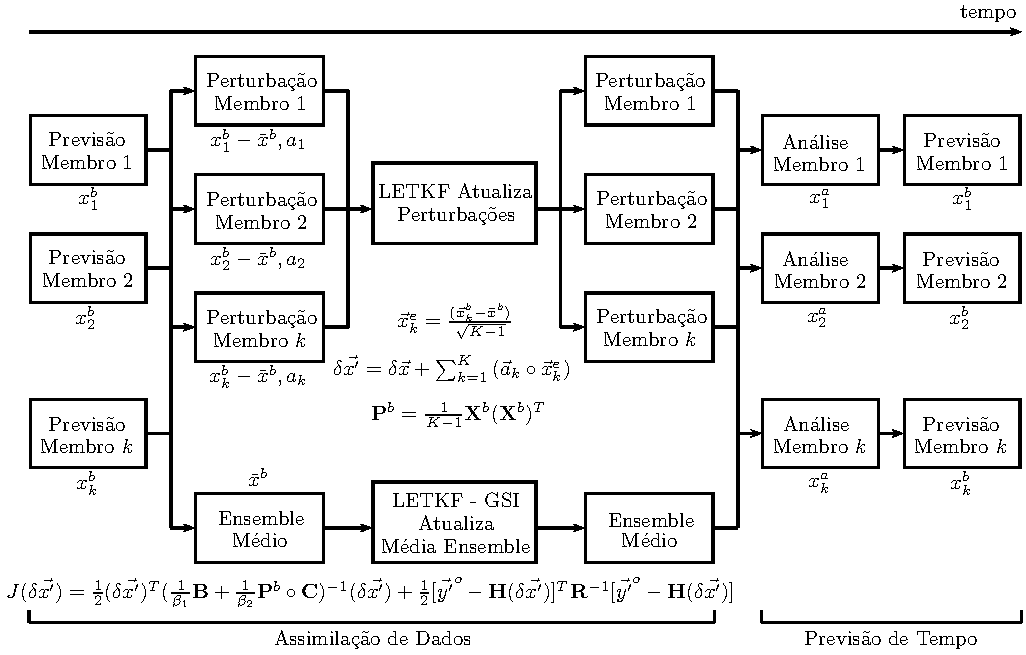
\includegraphics[scale=0.45]{./figs/diagrama_hibrido_novo_pt-tempos.pdf}
				\caption{Exemplo de um diagrama produzido no programa \LaTeX\textit{Draw}.}
		\end{figure}
	\end{block}
\end{frame}

\section{Parte I - Preparação}

\subsection{Escolhendo e Instalando o Compilador}

\begin{frame}{Escolhendo e Instalando o Compilador}
O \LaTeX{} é uma linguagem de marcação que é interpretada por um \textbf{compilador} que se encarrega de mostrar o resultado em um arquivo final.
    \pause
	\begin{block}{Compiladores}
		\begin{itemize}
			\item Linux: \TeX{}\textit{Live}
			\item \textit{Microsoft Windows}: \TeX{}\textit{Live}
			\item Mac OS: Mac\TeX{}
		\end{itemize}
	\end{block}
\end{frame}

\begin{frame}[fragile]{Escolhendo e Instalando o Compilador}
\begin{block}{Linux}
\vspace{0.5em}
No Linux, o \LaTeX{} pode ser facilmente instalado.
\begin{meucomandot}{Debian e derivados}
sudo apt install texlive-full
\end{meucomandot}
ou
\begin{meucomandot}{Red Hat e derivados}
sudo dnf install texlive-scheme-full
\end{meucomandot}
\end{block}
\end{frame}

\begin{frame}[fragile]{Escolhendo e Instalando o Compilador}
\begin{block}{\textit{Microsoft Windows}}
\vspace{0.5em}
No \textit{Microsoft Windows}, basta baixar e instalar o pacote \url{http://mirror.ctan.org/systems/texlive/tlnet/install-tl-windows.exe}
\end{block}

\begin{block}{Mac OS}
\vspace{0.5em}
No Mac OS, basta baixar e instalar o pacote \url{http://tug.org/cgi-bin/mactex-download/MacTeX.pkg} 
Pode-se também instalar pela linha de comando:
\begin{meucomandot}{Mac OS}
brew install caskroom/cask/brew-cask
brew cask install mactex
\end{meucomandot}
\end{block}
\end{frame}

\subsection{Compilação de um documento \LaTeX{}}

\begingroup
\setbeamercolor{background canvas}{bg=laranjainpe!90}
\begin{frame}[plain,fragile]{}
\begin{texexptitled}[center, enhanced jigsaw, width=.99\paperwidth, height=0.99\paperheight, middle=2mm, listing side comment, righthand width=5cm, compilable listing, run latex, run dvips, run ps2pdf, pdf comment, comment style={raster columns=1},freeze pdf]{Um documento \LaTeX{} mínimo}{exe_doc}
\documentclass[10pt]{article}
% Este é o preâmbulo
\usepackage[utf8]{inputenc}
\usepackage{lipsum}

\title{Título}
\author{Nome}
\date{\today}

% A partir daqui inicia-se o documento
\begin{document}
\maketitle

\section{Seção}

\lipsum[1-3]
\end{document}
\end{texexptitled}
\end{frame}
\endgroup

\begin{frame}{Compilação de um documento \LaTeX{}}
\tikzstyle{format} = [draw, thin, fill=blue!20]
\tikzstyle{medium} = [ellipse, draw, thin, fill=green!20, minimum height=2.5em]
\begin{figure}
\vspace{3em}
\begin{tikzpicture}[node distance=3cm, auto,>=latex', thick]
    % We need to set at bounding box first. Otherwise the diagram
    % will change position for each frame.
    \path[use as bounding box] (-1,0) rectangle (10,-2);
    \path[->]<1-> node[format] (tex) {arq. {\tt .tex}};
    \path[->]<2-> node[format, right of=tex] (dvi) {arq. {\tt .dvi}}
                  (tex) edge node {\LaTeX} (dvi);
    \path[->]<3-> node[format, right of=dvi] (ps) {arq. {\tt .ps}}
                  node[medium, below of=dvi] (screen) {visualização}
                  (dvi) edge node {dvips} (ps)
                        edge node[swap] {xdvi} (screen);
    \path[->]<4-> node[format, right of=ps] (pdf) {arq. {\tt .pdf}}
                  node[medium, below of=ps] (print) {impressão}
                  (ps) edge node {ps2pdf} (pdf)
                       edge node[swap] {gs} (screen)
                       edge (print);
    \path[->]<5-> (pdf) edge (screen)
                        edge (print);
    \path[->, draw]<6-> (tex) -- +(0,1) -| node[near start] {pdf\LaTeX} (pdf);
\end{tikzpicture}
\vspace{2.5em}
\visible<6>{\caption{Etapas envolvidas na compilação de um documento \LaTeX{}. Adaptado de \url{http://www.texample.net/tikz/examples/tex-workflow/}.}}
\end{figure}
\end{frame}

\begin{frame}{Compilação de um documento \LaTeX{}}
\vspace{-3em}
\begin{table}
\caption{Alguns tipos de compiladores \LaTeX{}.}
\vspace{-0.5em}
\begin{center}
    \begin{tabular}{p{2cm}p{8cm}}
    \toprule
    \textbf{Seção} & \textbf{Comando} \\
    \midrule
    \LaTeX{}    & Compilador \LaTeX{} puro, gera saída DVI, necessita do pacote {\tt inputenc} \\
    pdf\LaTeX{} & Compilador \LaTeX{} puro, gera saída em PDF, necessita do pacote {\tt inputenc} \\
    \XeLaTeX{}  & Compilador \LaTeX{} avançado, gera saída em PDF, não necessita do pacote {\tt inputenc}, suporta \textit{OpenType} \\
    Lua\LaTeX{} & Compilador \LaTeX{} avançado, gera saída em PDF, não necessita do pacote {\tt inputenc}, permite uso da linguagem Lua, suporta \textit{OpenType} \\
    \bottomrule
    \end{tabular}
\end{center}
\end{table}
\end{frame}

\begin{frame}{Compilação de um documento \LaTeX{}}
\begin{block}{Como a compilação é definida?}
\begin{itemize}
    \item Editor;
    \item Sistema operacional.
\end{itemize}
\end{block}
Na linha de comando (eg., Linux, MacOS ou \textit{Microsoft Windows}\footnote{Considerando-se que o \textit{Windows Subsystem for Linux} e o \LaTeX{} estão instalados.}) a compilação segue da seguinte forma:
\end{frame}

\begin{frame}[fragile]{Compilação de um documento \LaTeX{}}
	\vspace{-2em}
    \begin{block}{Linha de comando\footnote{Se for utilizado o compilador \XeLaTeX{}, o arquivo PDF será criado automaticamente. Além disso, estes comandos aceitam opções.}}
        \vspace{0.5em}
        \begin{meucomandot}{Documento simples}
            latex documento.tex
            dvips documento.dvi
            ps2pdf documento.ps
        \end{meucomandot}
    
        \begin{meucomandot}{Documento com referência Bib\TeX{}}
            latex documento.tex
            bibtex documento
            latex documento
            latex documento
        \end{meucomandot}
    \end{block}
\end{frame}

\section{Parte II - Entendendo o \LaTeX{}}

\begin{frame}[fragile]{Localização e acentos}
    \begin{block}{Pacotes de idiomas}
        \begin{itemize}
            \item \mintinline{latex}{\usepackage[brazilian]{babel}}
            \item \mintinline{latex}{\usepackage[utf8]{inputenc}}\footnote{Não é necessário nos compiladores \XeLaTeX{} e Lua\LaTeX{}; já está pré-carregado nas versões mais recentes do \LaTeX{}.} ou
            \item \mintinline{latex}{\usepackage[latin1]{inputenc}}\footnote{Em desuso, utilize apenas se no seu computador os arquivos são salvos com a codificação ``ISO8859'', ``Western (Latin 1)'' ou ``Windows Latin 1''. }
        \end{itemize}
    \end{block}
    \begin{block}{Pacote de escrita (acentos e hifenização)}
        \begin{itemize}
            \item \mintinline{latex}{\usepackage[T1]{fontenc}}
        \end{itemize}
    \end{block}
\end{frame}

\subsection{Caracteres, símbolos especiais e acentos}

\begin{frame}[fragile]{Caracteres Especiais \LaTeX{}}
\begin{block}{Caracteres especiais do \LaTeX{}}
\begin{multicols}{5}
    \begin{enumerate}
        \item $\backslash$
        \item \#
        \item \$
        \item \%
        \item \&
        \item \^{}
        \item \_
        \item \{
        \item \}
        \item \texttt{\~{}}
    \end{enumerate}
\end{multicols}
\end{block}
    \begin{texexptitled}[center lower,enhanced,middle=2mm,listing side text]{Marcação para caracteres especiais}{exe_caracesp}
        $\backslash$
        \\  
        \^{}
        \\
        \texttt{\~{}}
    \end{texexptitled}
\end{frame}

\begin{frame}[fragile]{Localização e acentos}
\begin{texexptitled}[center lower,enhanced,middle=2mm,listing side text,righthand width=2.5cm]{Uso de acentos latinos no \LaTeX{}}{exe_acentos}
\'A \'E \'I \'O \'U

\'a \'e \'i \'o \'u

\^a \^A \~a \~A \`a \`A \~o \~O

\^e \^E \^o \^O

\"u \"U

\c{c} \c{C}
\end{texexptitled}
\end{frame}

\subsection{Tipos, tamanhos e estilos de letras}

\begin{frame}[fragile]{Tipos, tamanhos e estilos de letras}
\begin{texexptitled}[center lower, enhanced, middle=2mm, listing side text, righthand width=2cm]{Marcações mais comuns em fontes}{exe_estilos}
\textit{itálico}       \\
\textsl{inclinado}     \\
\underline{sublinhado} \\
\textbf{negrito}       \\
\textsuperscript{o}C   \\
H\textsubscript{2}O
\end{texexptitled}
\end{frame}

\begin{frame}[fragile]{Tipos, tamanhos e estilos de letras}
\begin{texexptitled}[center lower, enhanced, middle=2mm, listing side text, righthand width=2cm]{Tamanhos de fontes}{exe_tamfonte}
{\Huge Huge} \\
{\huge huge} \\
{\LARGE LARGE} \\
{\Large Large} \\
{\large large} \\
{\normalsize normalsize} \\
{\small small} \\
{\footnotesize footnotesize} \\
{\scriptsize scriptsize} \\
{\tiny tiny}
\end{texexptitled}
\end{frame}

\begin{frame}[fragile]{Tipos, tamanhos e estilos de letras}
\begin{texexptitled}[center lower,enhanced,middle=2mm]{Texto com diferentes tamanhos de fontes}{exe_tamfontefrase}
À noite, vovô {\large Kowalsky} vê o {\huge ímã} cair no {\small pé} do pinguim {\Huge queixoso} e vovó põe açúcar no {\footnotesize chá} de {\tiny tâmaras} do jabuti feliz. 
\end{texexptitled}
\end{frame}

\begin{frame}[fragile]{Tipos, tamanhos e estilos de letras}
\begin{texexptitled}[center lower,enhanced,middle=2mm]{Estilos de fontes, máquina de escrever ({\tt texttt})}{exe_font1}
\texttt{Máquina de Escrever} | \texttt{\textit{Máquina de Escrever, em itálico}} | \texttt{\textsl{Máquina de Escrever, inclinado}}
\end{texexptitled}
\end{frame}

\begin{frame}[fragile]{Tipos, tamanhos e estilos de letras}
\begin{texexptitled}[center lower,enhanced,middle=2mm]{Estilos de fontes, sem serifa ({\tt textsf})}{exe_font2}
\textsf{Sem Serifa} | \textsf{\textit{Sem Serifa, em itálico}} | \textsf{\textsl{Sem Serifa, inclinado}}
\end{texexptitled}
\end{frame}

\begin{frame}[fragile]{Tipos, tamanhos e estilos de letras}
\begin{texexptitled}[center lower,enhanced,middle=2mm]{Estilos de fontes, com serifa ({\tt textrm})}{exe_font3}
\textrm{Com Serifa, estilo Romano} | \textrm{\textit{Com Serifa, estilo Romano itálico}} | \textrm{\textsl{Com Serifa, estilo Romano inclinado}}
\end{texexptitled}
\end{frame}

\subsection{Títulos e Seções}

\begin{frame}{Títulos e Seções}
\begin{table}
\caption{Títulos e Seções\footnote{Nem todas as classes possuem todas as seções. {\tt part} e {\tt chapter} funcionam apenas com as classes {\tt book} e {\tt report}.}}
\begin{center}
    \begin{tabular}{p{3cm}p{3cm}c}
    \toprule
    \textbf{Seção} & \textbf{Comando}                & \textbf{Nível} \\
    \midrule
    Parte          & \mintinline{latex}{\part}       & -1             \\
    Capítulo       & \mintinline{latex}{\chapter}    & 0              \\
    Seção          & \mintinline{latex}{\section}    & 1              \\
    Subseção       & \mintinline{latex}{\subsection} & 2              \\
    Parágrafo      & \mintinline{latex}{\par}        & 3              \\
    Subparágrafo   & \mintinline{latex}{\subpar}     & 4              \\
    \bottomrule
    \end{tabular}
\end{center}
\end{table}
\end{frame}

\subsection{Cores, Paletas e Cores Customizadas}

\begin{frame}[fragile]{Cores, Paletas e Cores Customizadas}
    \begin{block}{Paleta de cores padrão\footnote{Estas cores são fornecidas pelo pacote {\tt xcolor}.} do \LaTeX{}}
        \begin{center}
            \scalebox{0.7}{
                \begin{tikzpicture}
                    \fill [black] (0,0) rectangle ++(1.15,1.15);
                    \draw (0.615,-0.4) node {black};
                    \fill [blue] (1.75,0) rectangle ++(1.15,1.15);
                    \draw (2.365,-0.4) node {blue};
                    \fill [brown] (3.5,0) rectangle ++(1.15,1.15);
                    \draw (4.115,-0.4) node {brown};
                    \fill [cyan] (5.25,0) rectangle ++(1.15,1.15);
                    \draw (5.865,-0.4) node {cyan};
                    \fill [darkgray] (7,0) rectangle ++(1.15,1.15);
                    \draw (7.615,-0.4) node {darkgray};
                    \fill [gray] (8.75,0) rectangle ++(1.15,1.15);
                    \draw (9.365,-0.4) node {gray};
                    \fill [green] (10.5,0) rectangle ++(1.15,1.15);
                    \draw (11.115,-0.4) node {green};
                    \fill [lime] (12.25,0) rectangle ++(1.15,1.15);
                    \draw (12.865,-0.4) node {lime};
                    \fill [magenta] (14,0) rectangle ++(1.15,1.15);
                    \draw (14.615,-0.4) node {magenta};
                    
                    \fill [olive] (0,-1) rectangle ++(1.15,-1.15);
                    \draw (0.615,-2.65) node {olive};
                    \fill [orange] (1.75,-1) rectangle ++(1.15,-1.15);
                    \draw (2.365,-2.65) node {orange};
                    \fill [pink] (3.5,-1) rectangle ++(1.15,-1.15);
                    \draw (4.115,-2.65) node {pink};
                    \fill [purple] (5.25,-1) rectangle ++(1.15,-1.15);
                    \draw (5.865,-2.65) node {purple};
                    \fill [red] (7,-1) rectangle ++(1.15,-1.15);
                    \draw (7.615,-2.65) node {red};
                    \fill [teal] (8.75,-1) rectangle ++(1.15,-1.15);
                    \draw (9.365,-2.65) node {teal};
                    \fill [violet] (10.5,-1) rectangle ++(1.15,-1.15);
                    \draw (11.115,-2.65) node {violet};
                    \draw[fill=white] (12.25,-1) rectangle ++(1.15,-1.15);
                    \draw (12.865,-2.65) node {white};
                    \fill [yellow] (14,-1) rectangle ++(1.15,-1.15);
                    \draw (14.615,-2.65) node {yellow};
                \end{tikzpicture}
            }
        \end{center}
    \end{block}
\end{frame}

\begin{frame}[fragile]{Cores, Paletas e Cores Customizadas}
\begin{texexptitled}[center lower,enhanced,middle=2mm]{Texto com fundo colorido, paleta padrão}{exe_cor3}
\textit{\colorbox{pink}{Quem} \colorbox{cyan}{traz} \colorbox{green}{CD}, \colorbox{olive}{LP}, \colorbox{violet}{\color{white}{fax}}, \colorbox{blue}{\color{white}{engov}} \colorbox{red}{e} \colorbox{lime}{whisky} \colorbox{orange}{JB?}}
\end{texexptitled}
\end{frame}

\begin{frame}[fragile]{Cores, Paletas e Cores Customizadas}
\begin{texexptitled}[center lower,enhanced,middle=2mm]{Definindo cores personalizadas}{exe_cor4}
\definecolor{meuazul1}{HTML}{0066ff}
\definecolor{meuazul2}{rgb}{0.2,0.6,1}
\definecolor{meuazul3}{RGB}{0,204,255}
\definecolor{meuazul4}{cmyk}{0.6,0,0,0}

\textit{Quem traz \colorbox{meuazul1}{\color{white}{CD}}, \colorbox{meuazul2}{\color{white}{LP}}, \colorbox{meuazul3}{\color{white}{fax}}, \colorbox{meuazul4}{\color{white}{engov}} e whisky JB?}
\end{texexptitled}
\end{frame}

\subsection{Unidades, Medidas e Macros de Medidas}

\begin{frame}{Unidades, Medidas e Macros de Medidas}
\begin{table}
\centering
\caption{Unidades de Medidas mais Comuns no \LaTeX{}.}
    \begin{tabular}{p{3cm}cc}
    \toprule
    \textbf{Unidade} & \textbf{Abreviação} & \textbf{Valor em Pontos}              \\
    \midrule
    Ponto            & {\tt pt}.           & 1 {\tt pt}                            \\
    Milímetro        & {\tt mm}.           & 1 {\tt mm} = 2,84 {\tt pts}           \\
    Centímetro       & {\tt cm}.           & 1 {\tt cm} = 28,4 {\tt pts}           \\
    Polegada         & {\tt in}.           & 1 {\tt in} = 72,27 {\tt pts}          \\
    Paica             & {\tt pc}.           & 1 {\tt pc} = 12 {\tt pts}            \\
    Altura de ``x''  & {\tt ex}.           & \textit{Depende da fonte utilizada}   \\
    Altura de ``M''  & {\tt em}.           & \textit{Depende da fonte utilizada}   \\
    \bottomrule
    \end{tabular}
\end{table}
\end{frame}

\begin{frame}{Unidades, Medidas e Macros de Medidas}
\begin{table}
	\centering
	\caption{Algumas Macros de Medidas do \LaTeX{}.}
	\vspace{-1em}
	\begin{tabular}{p{2.5cm} p{7.5cm}}
		\toprule
		\textbf{Macro}                    & \textbf{Descrição}                                 \\
		\midrule
		\mintinline{latex}{\paperwidth}   & Largura de uma página                              \\
		\mintinline{latex}{\paperheight}  & Altura de uma página                               \\
		\mintinline{latex}{\textheight}   & Altura do texto na página                          \\
		\mintinline{latex}{\textwidth}    & Largura do texto na página                         \\
		\mintinline{latex}{\parindent}    & Indentação de um parágrafo                         \\
		\mintinline{latex}{\parskip}      & Espaçamento extra entre parágrafos                 \\
		\mintinline{latex}{\baselineskip} & Distância vertical entre as linhas em um parágrafo \\
		\mintinline{latex}{\columnsep}    & Distância entre colunas de texto                   \\
		\mintinline{latex}{\columnwidth}  & Largura de uma coluna de texto                     \\
		\mintinline{latex}{\linewidth}    & Largura de uma linha em um ambiente local          \\
		\bottomrule
		\label{tab:medidas}
	\end{tabular}
\end{table}
\end{frame}

\begingroup
\setbeamercolor{background canvas}{bg=laranjainpe!90}
\begin{frame}[plain,fragile]{}
\begin{texexptitled}[center, width=0.99\paperwidth, height=0.99\paperheight, enhanced jigsaw, middle=2mm, listing side comment, righthand width=3.25cm, compilable listing, run latex, run dvips, run ps2pdf, pdf comment, comment style={raster columns=1}, freeze pdf]{Largura relativa com a \textit{macro} {\tt textwidth}}{exe_meds1}
\documentclass{article}
\usepackage[utf8]{inputenc}
\usepackage{lipsum}
\usepackage{graphicx}
\title{Título}
\author{Nome}
\date{\today}
\begin{document}
\maketitle
\section{Uma Seção}
\lipsum[2]
\includegraphics[width=1.0\textwidth]
{example-image-a}
\lipsum[3]
\includegraphics[width=0.5\textwidth]
{example-image-b}
\end{document}
\end{texexptitled}
\end{frame}
\endgroup

\begin{frame}{Unidades, Medidas e Macros de Medidas}
\vspace{0.75em}
\begin{table}
\centering
\caption{Algumas Macros de Espaçamento do \LaTeX{}.}
    \vspace{-1.5em}
    \begin{tabular}{p{2cm}p{8cm}}
    \toprule
    \textbf{Macro} & \textbf{Descrição} \\
    \midrule
    \mintinline{latex}{\hspace}    & Adiciona espaço horizontal (pode utilizar qualquer unidade da Tabela \ref{tab:medidas}, incluindo valores negativos)     \\
    \mintinline{latex}{\vspace}    & Adiciona espaço vertical (pode utilizar qualquer unidade da Tabela \ref{tab:medidas}, incluindo valores negativos)       \\
    \mintinline{latex}{\smallskip} & Equivalente a \mintinline{latex}{\vspace{smallskipamount}}, onde {\tt smallskipamount} é relativo ao estilo do documento \\
    \mintinline{latex}{\medskip}   & Equivalente a \mintinline{latex}{\vspace{medskipamount}}, onde {\tt medskipamount} é relativo ao estilo do documento     \\
    \mintinline{latex}{\bigskip}   & Equivalente a \mintinline{latex}{\vspace{bigskipamount}}, onde {\tt bigskipamount} é relativo ao estilo do documento     \\
    \bottomrule
    \end{tabular}
\end{table}
\end{frame}

\subsection{Parágrafos, Alinhamentos e Espaçamentos}

\begin{frame}[fragile]{Parágrafos, Alinhamentos e Espaçamentos}
\begin{texexptitled}[enhanced,middle=2mm]{Parágrafos sem quebra de linha}{exe_par1}
\lipsumsentence[1-4] 
\lipsumsentence[5-8]
\end{texexptitled}
\end{frame}

\begin{frame}[fragile]{Parágrafos, Alinhamentos e Espaçamentos}
\begin{texexptitled}[enhanced,middle=2mm]{Parágrafos com quebra de linha, separados por uma linha em branco}{exe_par2}
\lipsumsentence[1-4]

\lipsumsentence[5-8]
\end{texexptitled}
\end{frame}

\begin{frame}[fragile]{Parágrafos, Alinhamentos e Espaçamentos}
\begin{texexptitled}[enhanced,middle=2mm]{Parágrafos com quebra de linha, separados por duas barras invertidas (\mintinline{latex}{\\})}{exe_par3}
\lipsumsentence[1-4] \\
\lipsumsentence[5-8]
\end{texexptitled}
\end{frame}

\begin{frame}[fragile]{Parágrafos, Alinhamentos e Espaçamentos}
\begin{texexptitled}[enhanced,middle=2mm]{Parágrafos separados pelo comando {\tt newline}}{exe_par4}
\lipsumsentence[1-4]
\newline
\lipsumsentence[5-8]
\end{texexptitled}
\end{frame}

\begin{frame}[fragile]{Parágrafos, Alinhamentos e Espaçamentos}
\begin{texexptitled}[enhanced,middle=2mm]{Novo parágrafo iniciado pelo comando {\tt par}}{exe_par5}
\lipsumsentence[1-4] \par
\lipsumsentence[5-8]
\end{texexptitled}
\end{frame}

\begin{frame}[fragile]{Parágrafos, Alinhamentos e Espaçamentos}
\begin{texexptitled}[enhanced,middle=2mm]{Novo parágrafo iniciado pelo comando {\tt par}, com recuo especial}{exe_par6}
\setlength{\parindent}{3em}

\lipsumsentence[1-4] \par
\lipsumsentence[5-8]
\end{texexptitled}
\end{frame}

\begin{frame}[fragile,plain]{Parágrafos, Alinhamentos e Espaçamentos}
\begin{texexptitled}[enhanced,middle=2mm]{Novo parágrafo iniciado pelo comando {\tt par}, com recuo ({\tt parindent}) e espaçamento ({\tt parskip}) especiais}{exe_par7}
\setlength{\parindent}{3em}
\setlength{\parskip}{1em}

\lipsumsentence[1-4] \par
\lipsumsentence[5-8]
\end{texexptitled}
\end{frame}

\begingroup
\setbeamercolor{background canvas}{bg=laranjainpe!90}
\begin{frame}[plain,fragile]{}
\begin{texexptitled}[center,width=0.99\paperwidth,height=0.99\paperheight,enhanced jigsaw,middle=2mm,listing side comment,righthand width=4cm,compilable listing,run latex,run dvips,run ps2pdf,pdf comment,comment style={raster columns=1},freeze pdf]{Espaçamento de linha simples ({\tt baselinestretch, 1.0})}{exe_par8}
\documentclass{article}
\usepackage[utf8]{inputenc}
\usepackage{lipsum}

\renewcommand{
\baselinestretch}{1.0}

\begin{document}

\setlength{\parindent}{3em}
\setlength{\parskip}{1em}
\lipsum[1] \par
\lipsum[2]

\end{document}
\end{texexptitled}
\end{frame}
\endgroup

\begingroup
\setbeamercolor{background canvas}{bg=laranjainpe!90}
\begin{frame}[plain,fragile]{}
\begin{texexptitled}[center,width=0.99\paperwidth,height=0.99\paperheight,enhanced jigsaw,middle=2mm,listing side comment,righthand width=4cm,compilable listing,run latex,run dvips,run ps2pdf,pdf comment,comment style={raster columns=1},freeze pdf]{Espaçamento de linha médio ({\tt baselinestretch, 1.3})}{exe_par9}
\documentclass{article}
\usepackage[utf8]{inputenc}
\usepackage{lipsum}

\renewcommand{
\baselinestretch}{1.3}

\begin{document}

\setlength{\parindent}{3em}
\setlength{\parskip}{1em}
\lipsum[1] \par
\lipsum[2]

\end{document}
\end{texexptitled}
\end{frame}
\endgroup

\begingroup
\setbeamercolor{background canvas}{bg=laranjainpe!90}
\begin{frame}[plain,fragile]{}
\begin{texexptitled}[center,width=0.99\paperwidth,height=0.99\paperheight,enhanced jigsaw,middle=2mm,listing side comment,righthand width=4cm,compilable listing,run latex,run dvips,run ps2pdf,pdf comment,comment style={raster columns=1},freeze pdf]{Espaçamento de linha duplo ({\tt baselinestretch, 1.6})}{exe_par10}
\documentclass{article}
\usepackage[utf8]{inputenc}
\usepackage{lipsum}

\renewcommand{
\baselinestretch}{1.6}

\begin{document}

\setlength{\parindent}{3em}
\setlength{\parskip}{1em}
\lipsum[1] \par
\lipsum[2]

\end{document}
\end{texexptitled}
\end{frame}
\endgroup

\begin{frame}[fragile]{Parágrafos, Alinhamentos e Espaçamentos}
\begin{texexptitled}[enhanced,middle=2mm]{Parágrafos centralizados, utilizando o ambiente \mintinline{latex}{center}}{exe_par11}
\begin{center}
\lipsumsentence[9-10] \\ 
\lipsumsentence[11-12]
\end{center}
\end{texexptitled}
\end{frame}

\begin{frame}[fragile]{Parágrafos, Alinhamentos e Espaçamentos}
\begin{texexptitled}[enhanced,middle=2mm]{Parágrafos alinhados à esquerda, utilizando o ambiente {\tt flushleft}}{exe_par12}
\begin{flushleft}
\lipsumsentence[9-10] \\ 
\lipsumsentence[11-12]
\end{flushleft}
\end{texexptitled}
\end{frame}

\begin{frame}[fragile]{Parágrafos, Alinhamentos e Espaçamentos}
\begin{texexptitled}[enhanced,middle=2mm]{Parágrafos alinhados à direita, utilizando o ambiente {\tt flushright}}{exe_par13}
\begin{flushright}
\lipsumsentence[9-10] \\ 
\lipsumsentence[11-12]
\end{flushright}
\end{texexptitled}
\end{frame}

\subsection{Notas de rodapé}

\begin{frame}[fragile]{Notas de rodapé}
\begin{texexptitled}[enhanced,middle=2mm]{Nota de rodapé, utilizando o marcador {\tt footnote}}{exe_rodape1}
À noite, vovô Kowalsky\footnote{Esta é uma nota de rodapé.} vê o ímã cair no pé do pinguim queixoso e vovó põe açúcar no chá de tâmaras do jabuti feliz\footnote{Este é uma outra nota de rodapé.}.
\end{texexptitled}
\end{frame}

\begin{frame}[fragile]{Notas de rodapé}
\begingroup
\renewcommand*{\thefootnote}{\alph{footnote}}
\begin{texexptitled}[enhanced,middle=2mm]{Nota de rodapé, utilizando os marcadores {\tt footnotemark} e {\tt footnotetext}}{exe_rodape2}
À noite, vovô Kowalsky vê o ímã\footnotemark[1] cair no pé do pinguim queixoso\footnotemark[2] e vovó põe açúcar no chá de tâmaras do jabuti feliz.

\footnotetext[1]{Esta é uma nota de rodapé.}
\footnotetext[2]{Esta é uma outra nota de rodapé.}
\end{texexptitled}
\endgroup
\end{frame}

\subsection{Listas Ordenadas e Não Ordenadas}

\begin{frame}[fragile]{Listas Ordenadas e Não Ordenadas}
\begin{texexptitled}[enhanced, listing side text, righthand width=4cm]{Lista não ordenada utilizando o ambiente \mintinline{latex}{itemize}}{exe_lista1}
\begin{itemize}
    \item Item 1
    \item Item 2
    \item Item 3
\end{itemize}
\end{texexptitled}
\end{frame}

\begin{frame}[fragile]{Listas Ordenadas e Não Ordenadas}
\begin{texexptitled}[enhanced, listing side text, righthand width=4cm]{Lista não ordenada utilizando o ambiente \mintinline{latex}{itemize} com símbolos diferentes}{exe_lista_simb1}
    \begin{itemize}
        \item[\#]    Item 1
        \item[--]    Item 2
        \item[@]     Item 3
        \item[$\to$] Item 4
    \end{itemize}
\end{texexptitled}
\end{frame}

\begin{frame}[fragile]{Listas Ordenadas e Não Ordenadas}
\begingroup
%\renewcommand{\labelenumi}{\arabic{enumi}.}
\begin{texexptitled}[enhanced, listing side text, righthand width=4cm]{Lista ordenada utilizando o ambiente \mintinline{latex}{enumerate}}{exe_lista3}
\begin{enumerate}
    \item Item 1
    \item Item 2
    \item Item 3
\end{enumerate}
\end{texexptitled}
\endgroup
\end{frame}

\subsection{Figuras e Ambientes de Figuras}

\begin{frame}[fragile,plain]{Figuras e Ambientes de Figuras}
\begin{texexptitled}[center, enhanced, middle=2mm]{Incorporando uma figura com o comando {\tt includegraphics} dentro do ambiente {\tt figure}}{exe_ambfig}
\begin{figure}[H]
    \caption{Uma figura dentro do ambiente {\tt figure}.}
    \includegraphics[width=3cm]{example-image-a}
\end{figure}
\end{texexptitled}
\end{frame}

\begin{frame}[fragile]{Figuras e Ambientes de Figuras}
\vspace{-1.5em}
\begin{table}
\centering
\caption{Opções de posicionamento\footnote{Pode-se utilizar também os ambientes {\tt center}, {\tt flushleft} e {\tt flushright} para posicionar as figuras dentro do ambiente {\tt figure}.} relativo do ambiente {\tt figure}.}
\vspace{-1em}
\label{tab:ambfig}
    \begin{tabular}{p{2cm}p{8cm}}
    \toprule
    \textbf{Opção} & \textbf{Descrição} \\
    \midrule
    {\tt h} & ``aqui'' (\textit{here}). Posição exata pode variar de acordo com outros elementos \\
    {\tt t} & ``topo'' da página (\textit{top}) \\
    {\tt b} & ``base'' da página (\textit{bottom}) \\
    {\tt p} & ``página'' separada (\textit{page}) \\
    {\tt !} & Força a posição onde o ambiente se encontra (e.g., {\tt h!}) \\
    {\tt H} & Precisamente no local (depende do pacote {\tt float}; equivalente a {\tt h!}) \\
    \bottomrule
    \end{tabular}
\end{table}
\end{frame}

\subsection{Matemática e Ambientes de Equações}

\begin{frame}[fragile]{Matemática e Ambientes de Equações}
\vspace{-1.5em}
\begin{texexptitled}[center lower,enhanced,middle=2mm]{Inserindo equações em linha (\textit{inline})}{exe_eq0}
Uma equação do segundo grau tem a forma geral, $ax^2 + bx + c =0$. Suas raízes são calculadas por, $x = \frac{-b \pm \sqrt{b^2 - 4ac}}{2a}$.
\end{texexptitled}
\end{frame}

\begin{frame}[fragile,plain]{Matemática e Ambientes de Equações}
\vspace{-1.5em}
\begin{texexptitled}[center lower,enhanced,middle=2mm]{Ambientes {\tt equation} e {\tt equation*}}{exe_eq1}
\begin{equation*}
x = \frac{-b \pm \sqrt{b^{2} - 4ac}}{2a}
\end{equation*}

\begin{equation}
\label{eq1}
x = \frac{-b \pm \sqrt{b^{2} - 4ac}}{2a}
\end{equation}
\end{texexptitled}
\end{frame}

\begin{frame}[fragile]{Matemática e Ambientes de Equações}
\begin{texexptitled}[center lower,enhanced,middle=2mm]{Ambientes {\tt equation} e {\tt split}}{exe_eq2}
\begin{equation*}
\begin{split}
f(x) & = x^{-\frac{1}{2}}   \\
     & = \frac{1}{\sqrt{x}}\text{, }\forall x \neq 0.
\end{split}
\end{equation*}
\end{texexptitled}
\end{frame}

\begin{frame}[fragile,plain]{Matemática e Ambientes de Equações}
\begin{texexptitled}[center,enhanced,middle=2mm]{Ambiente {\tt multline}}{exe_eq3}
\begin{multline*}
A(x,y)\frac{\partial^2{\Psi}}{\partial{x^2}} + B(x,y)\frac{\partial^2{\Psi}}{\partial{x}\partial{y}} + C(x,y)\frac{\partial^2{\Psi}}{\partial{y^2}} + D(x,y)\frac{\partial{\Psi}}{\partial{x}} + \\ + E(x,y)\frac{\partial{\Psi}}{\partial{y}} + F(x,y)\Psi = G(x,y)
\end{multline*}
\end{texexptitled}
\end{frame}

\begin{frame}[fragile]{Matemática e Ambientes de Equações}
\begin{texexptitled}[center lower,enhanced,middle=2mm]{Ambiente {\tt align}}{exe_eq4}
\begin{align*}
e^{i\pi} + 1 & = 0 \\ 
           e & = \lim_{n \to \infty}{\Bigg(1 + \frac{1}{n}\Bigg)^{n}}  
\end{align*}
\end{texexptitled}
\end{frame}

\begin{frame}[fragile]{Matemática e Ambientes de Equações}
\begin{texexptitled}[center lower,enhanced,middle=2mm]{Ambiente {\tt gather}}{exe_eq5}
\begin{gather*}
 x           = 1 + 2y + 3z \\ 
3x -  y + 2z = 0           \\
2x +  y      = 2 - z
\end{gather*}
\end{texexptitled}
\end{frame}

\subsection{Tabelas}

\begin{frame}[fragile]{Tabelas}
\begin{texexptitled}[center, enhanced, listing side text, righthand width=3cm, middle=2mm]{Exemplo de uma tabela simples com o ambiente {\tt tabular}}{exe_tab1}
\begin{tabular}{c c}
\toprule
\textbf{L0C1} & \textbf{L0C2} \\
\midrule
L1C1 & L1C2 \\
L2C1 & L2C2 \\
L3C1 & L3C2 \\
\bottomrule
\end{tabular}
\end{texexptitled}
\end{frame}

\begin{frame}[fragile,plain]{Tabelas}
\begin{texexptitled}[center, enhanced, middle=2mm]{Exemplo de uma tabela simples com o ambiente {\tt tabular} e colunas mais largas}{exe_tab3}
\begin{tabular}{p{3cm}  p{5cm}}
\toprule 
\textbf{L0C1} & \textbf{L0C2} \\
\midrule
L1C1 & L1C2 \\
L2C1 & L2C2 \\
L3C1 & L3C2 \\
\bottomrule
\end{tabular}
\end{texexptitled}
\end{frame}

\begin{frame}[fragile,plain]{Tabelas}
\begin{texexptitled}[center, enhanced, middle=2mm]{Exemplo de uma tabela simples utilizando o ambiente {\tt tabularx}}{exe_tab7}
\begin{tabularx}{\textwidth}{X | X | X}
\toprule
L0C1 & L0C2 & L0C3 \\
\midrule
L1C1 L1C1 & L1C2 L1C2 L1C2 L1C2 L1C2 L1C2 & L1C3 \\
L2C1 L2C1 & L2C2 L2C2 L2C2 L2C2 & L2C3 L2C3 \\
\bottomrule
\end{tabularx}
\end{texexptitled}
\end{frame}

\section{Parte III - Estilo do INPE}

\subsection{Obtendo do Estilo}

\begin{frame}{Obtendo o Estilo}
%\vspace{-0.25em}
\begin{block}{Entrar no \textit{site} \url{http://www.inpe.br/biblioteca/}}
  \begin{figure}[H]
    \begin{center}
        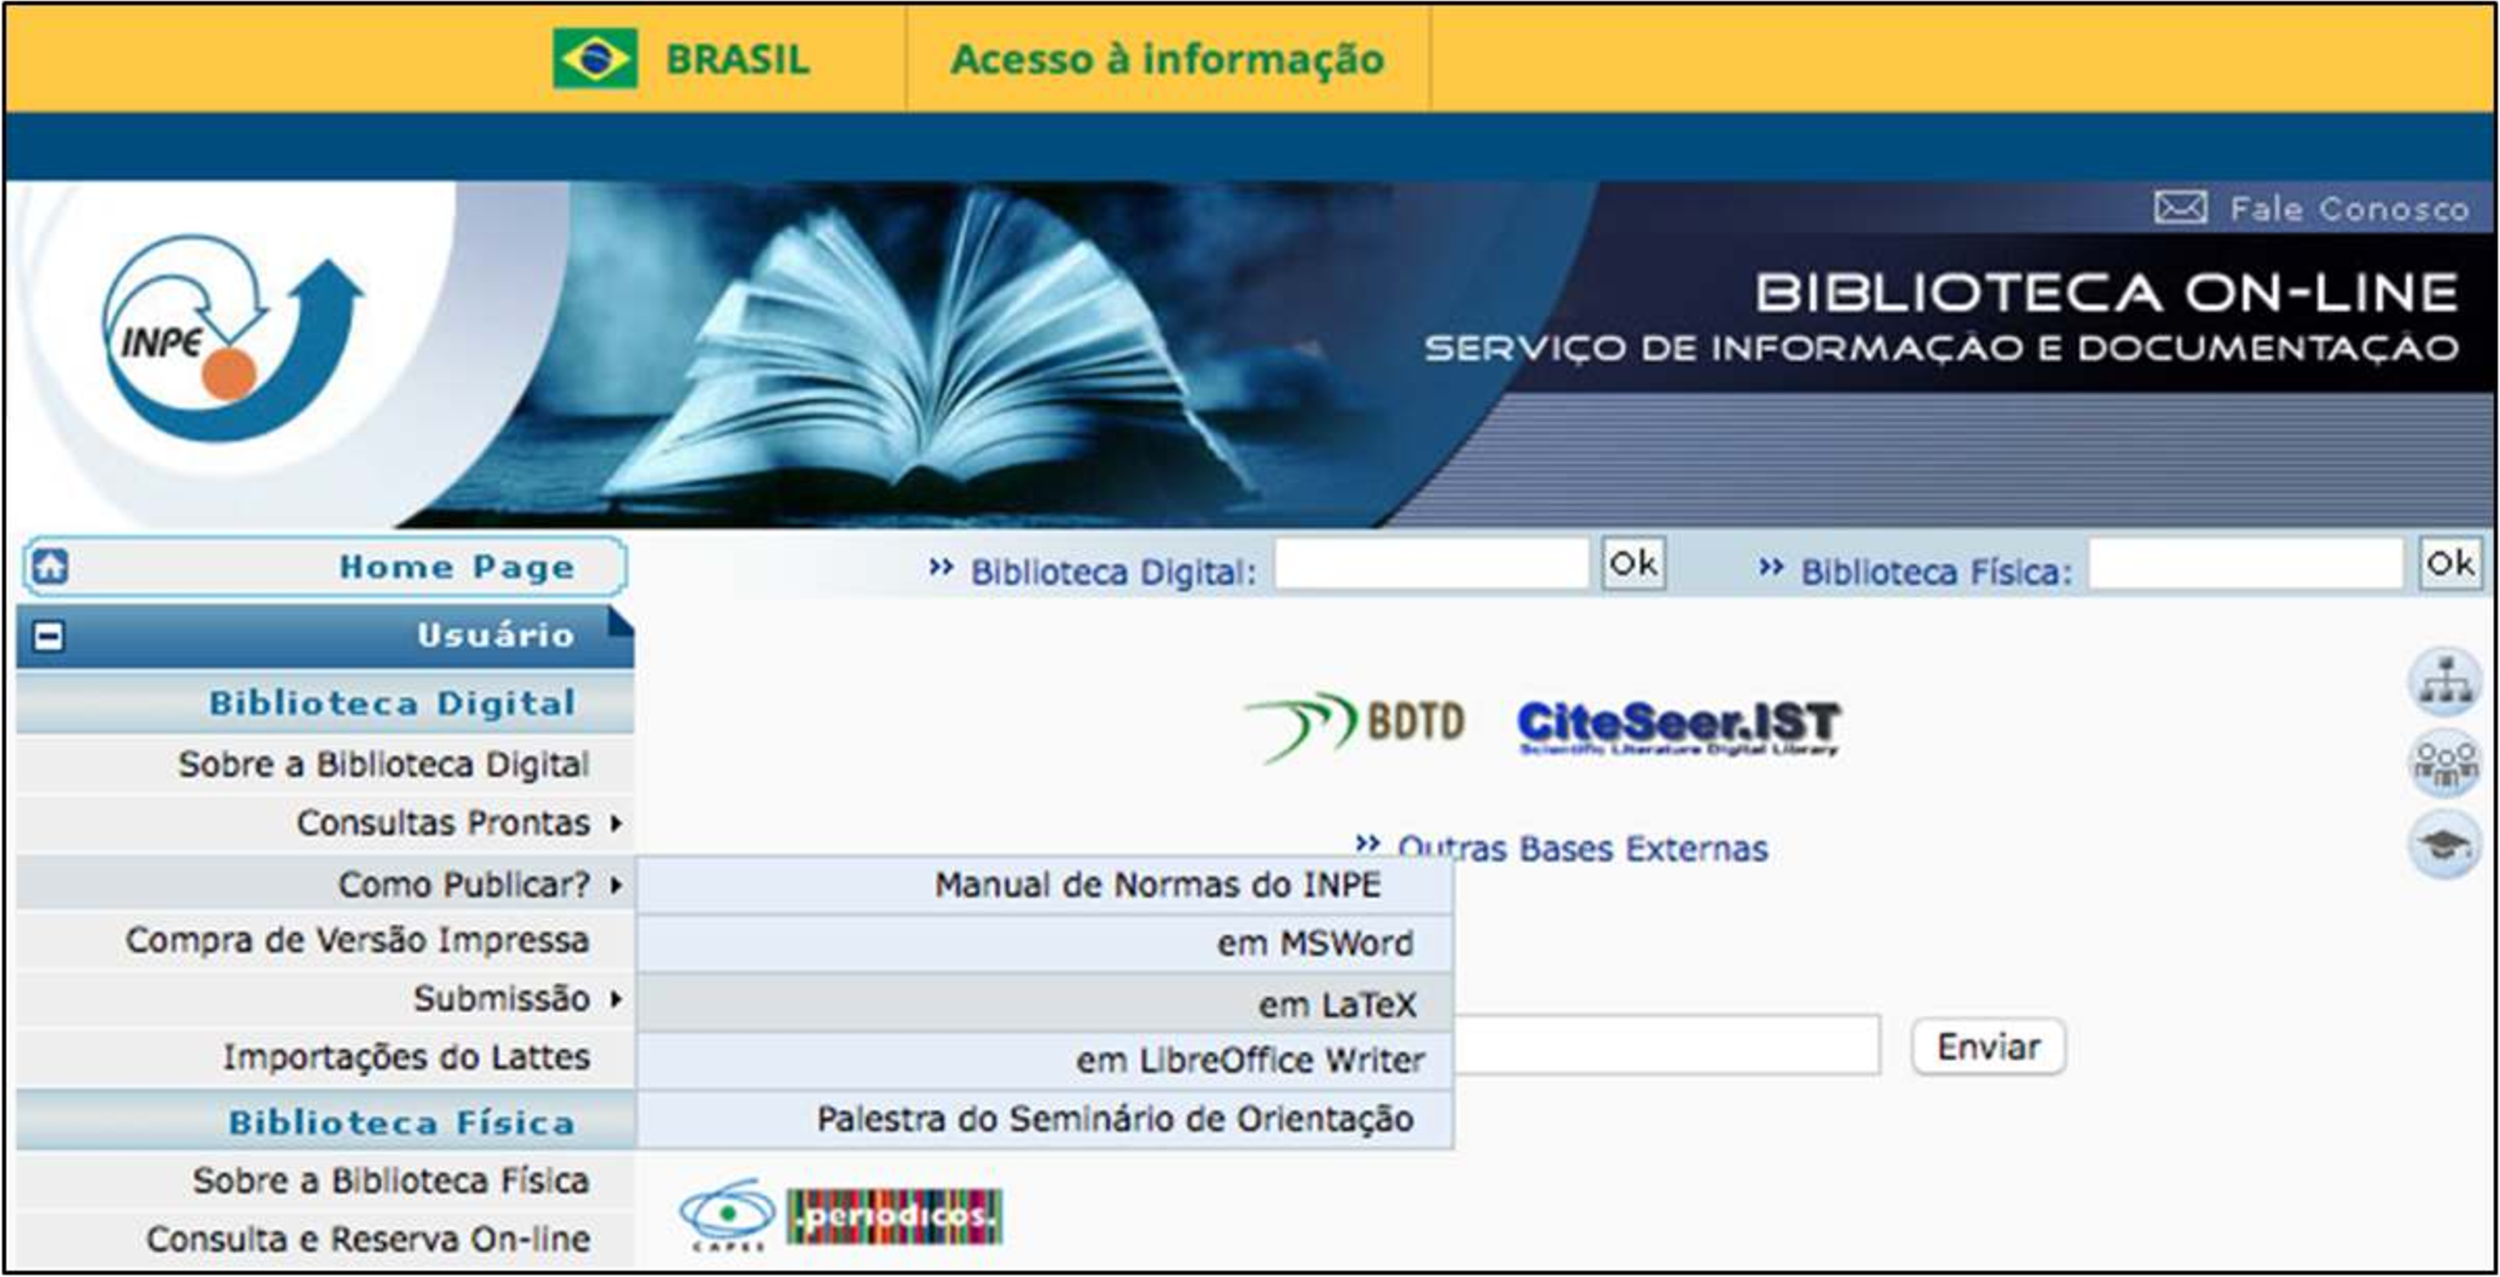
\includegraphics[scale=0.25]{./figs/biblio_pub_latex.pdf}
    \end{center}
    \caption{Obtenção do estilo \LaTeX{} do INPE a partir do \textit{site} da Biblioteca do INPE.}
  \end{figure}
\end{block}
\end{frame}

\subsection{Estrutura e Organização}

\begin{frame}[fragile]{Estrutura e Organização}
    \begin{block}{Arquivo {\tt archive.zip}}
        \vspace{1em}
        \begin{meucomandot}{Descompactar o arquivo (Linux/Mac OS)}
            unzip archive.zip
        \end{meucomandot}
        No \textit{Microsoft Windows}, basta clicar com o botão direito e clicar em ``Descompactar...''.
    \end{block}
\end{frame}

\begin{frame}{Estrutura e Organização}
\begin{figure}[H]
    %\vspace{1em}
    \begin{center}
        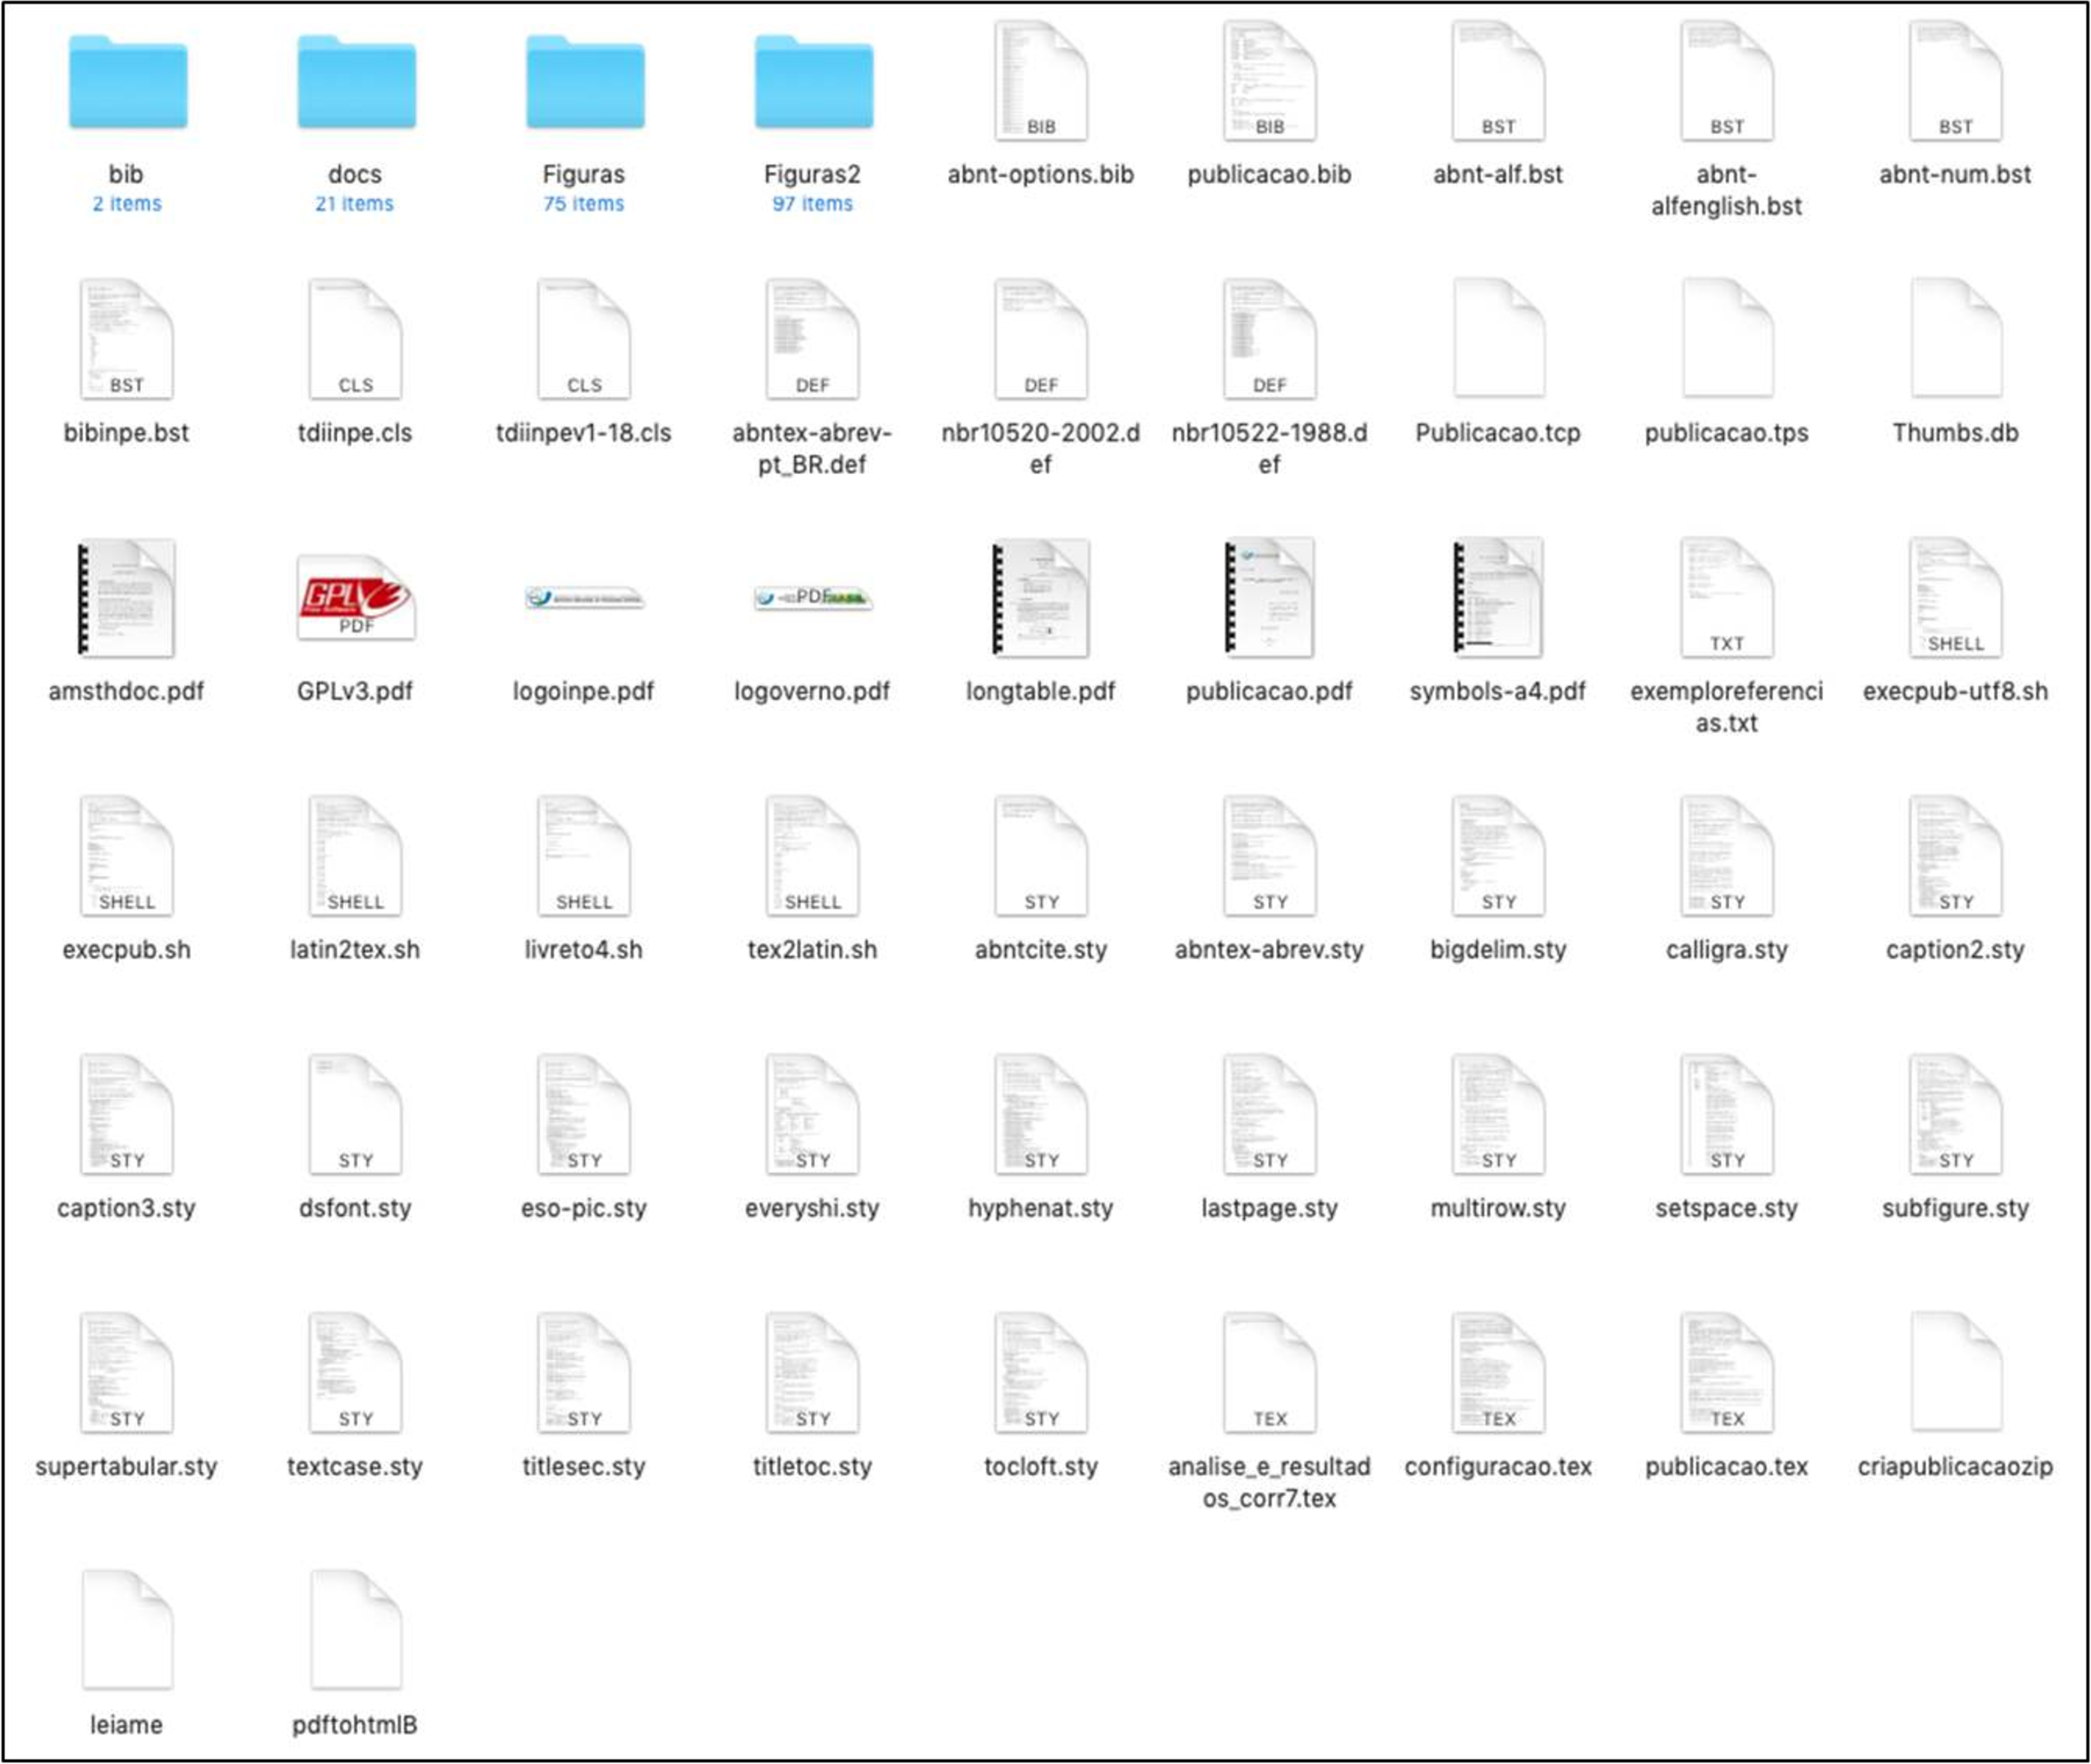
\includegraphics[scale=0.17]{./figs/estrutura_estilo_inpe.pdf}
    \end{center}
\caption{Estrutura e organização do estilo \LaTeX{} do INPE.}
\end{figure}
\end{frame}

\begin{frame}{Estrutura e Organização}
\settowidth{\leftmargini}{\usebeamertemplate{itemize item}}
\addtolength{\leftmargini}{\labelsep}
    \begin{multicols}{4}
    {\scriptsize
        \pause
         \faFolderOpen[regular]{} \textbf{Diretórios}
        \begin{enumerate}
            \item bib/
            \item Figuras/
            \item docs/
        \end{enumerate}
        \pause
        \faIcon*[regular]{file}{} \textbf{Arquivos do Estilo}
        \begin{enumerate}
            \color{azulinpe}{\item leiame
            \item GPLv3.pdf
            \item CCBY.png
            \item CCBYNC.png
            \item CCBYNCND.png
            \item CCBYNCSA.png
            \item CCBYND.png
            \item CCBYSA.png
            \item logoverno.pdf
            \item logoinpe.pdf
            \item tdiinpe.cls}                                                        
            \pause
            \color{laranjainpe}{\item abntex-abrev-pt\_BR.def      
            \item abntex-abrev.sty
            \item nbr10520-2002.def
            \item nbr10522-1988.def
            \item abnt-alf.bst
            \item abnt-alfenglish.bst
            \item bibinpe.bst
            \item eso-pic.sty
            \item abnt-num.bst
            \item abnt-options.bib
    		\item abntcite.sty}
        \end{enumerate}
        \pause
    	\faIcon*[regular]{file}{} \textbf{Outros Pacotes Fornecidos} 
    	\begin{enumerate}
            \item caption2.sty
            \item calligra.sty
            \item caption3.sty
    		\item hyphenat.sty
    		\item multirow.sty    
            \item dsfont.sty
    		\item supertabular.sty
    		\item tocloft.sty   
            \item setspace.sty
    		\item titlesec.sty   
            \item textcase.sty
    		\item lastpage.sty     
            \item bigdelim.sty
    		\item everyshi.sty 
            \item subfigure.sty
    		\item titletoc.sty
    	\end{enumerate}
        \pause
    	\faIcon*[regular]{file}{} \textbf{Arquivos de Configuração} 
    	\begin{itemize}
    		\item configuracao.tex
    	\end{itemize}
        \pause
        \faIcon*[regular]{file}{} \textbf{Arquivos de Documentos} 
        \begin{itemize}
            \item publicacao.tex
        \end{itemize}
        \pause
        \faFileCode[regular]{} \textbf{\textit{Scripts}} 
        \begin{enumerate}
            \item tex2latin.sh
            \item criapublicacaozip
            \item latin2tex.sh
            \item pdftohtmlB
            \item livreto4.sh
            \item execpub.sh
        \end{enumerate}
        \pause
        \faFilePdf[regular]{} \textbf{Documento Final} 
        \begin{itemize}
            \item publicacao.pdf
        \end{itemize}
    }
    \end{multicols}
\end{frame}

\begin{frame}{Estrutura e Organização}
    \begin{block}{\textit{Scripts} do estilo do INPE}
        \begin{itemize}
            \pause
            \item \textbf{criapublicacaozip}: \textit{script} que empacota o documento final ({\tt publicacao.pdf}) para publicação;
            \pause
            \item \textbf{latin2tex.sh}: \textit{script} que converte acentos latinos para a marcação da linguagem \LaTeX{};
            \pause
            \item \textbf{tex2latin.sh}: \textit{script} que converte acentos com marcação \LaTeX{} para acentos latinos;
            \pause
            \item \textbf{pdftohtmlB}: converte um documento PDF em HTML;
            \pause
            \item \textbf{livreto4.sh}: gera um livreto de quatro folhas no formato A4;
            \pause
            \item \textbf{execpub.sh}: gera o documento de saída ({\tt publicacao.pdf}) utilizando o compilador \LaTeX{}. 
        \end{itemize}       
    \end{block}
\end{frame}

\subsection{Arquivos de Configuração}

\begin{frame}{Arquivos de Configuração}
    \begin{block}{Arquivos principais}
        \begin{itemize}
            \item {\tt publicacao.tex}
            \item {\tt configuracao.tex}
        \end{itemize}
    \end{block}
\end{frame}

\begingroup
\setbeamercolor{background canvas}{bg=laranjainpe!90}
\begin{frame}[plain,fragile]{}
  \begin{meucomandolf}{Arquivo {\tt publicacao.tex}}
    \documentclass[
    % PARA ESCOLHER O ESTILO TIRE O SIMBOLO (COMENTÁRIO)
    %SemVinculoColorido,
    %SemFormatacaoCapitulo,
    %SemFolhaAprovacao,
    %SemImagens,
    %CitacaoNumerica, 
    %PublicacaoDissOuTese,
    %PublicacaoArtigoOuRelatorio,
    %PublicacaoProposta, 
    %PublicacaoLivro, 
    %PublicacaoLivro,SemFormatacaoCapitulo,
    english,portuguese, 
    %portuguese,english, 
    LogoINPE,
    CCBYNC,
    ]{tdiinpe}
    ...
  \end{meucomandolf}
\end{frame}

\begin{frame}[plain,fragile]{}
  \begin{meucomandolf}{Arquivo {\tt publicacao.tex} (Continuação)}
    ...
    %\watermark{Revisão No. ##} 
    \usepackage{rotating}
    \usepackage{dsfont}
    \usepackage{comment}
    
    \input{./configuracao} 
    
    \makeindex  
    ... 
    \marcaRegistrada{Informar aqui sobre marca registrada (a modificação desta linha deve ser feita no arquivo publicacao.tex).}
    \financiamento{Informar aqui sobre fontes financiadoras (a modificação desta linha deve ser feita no arquivo publicacao.tex).}
     
    \maketitle  
    ...
  \end{meucomandolf}
\end{frame}

\begin{frame}[plain,fragile]{}
  \begin{meucomandolf}{Arquivo {\tt publicacao.tex} (Continuação)}
    ...
    % Comente as linhas opcionais abaixo caso não as deseje
    \include{./docs/epigrafe} % Opcional
    \include{./docs/dedicatoria} % Opcional
    \include{./docs/agradecimentos} % Opcional
    \include{./docs/resumo} % Obrigatório
    \include{./docs/abstract} % Obrigatório
    
    \includeListaFiguras % Obrigatório (mais de 3 figuras)
    \includeListaTabelas % Obrigatório (mais de 3 tabelas)
    
    \include{./docs/abreviaturasesiglas} % Opcional
    \include{./docs/simbolos} % Opcional
    
    \includeSumario % Obrigatório
    \inicioIntroducao % Não altere este comando
    ...
  \end{meucomandolf}
\end{frame}

\begin{frame}[plain,fragile]{}
  \begin{meucomandolf}{Arquivo {\tt publicacao.tex} (Continuação)}
    ...
    \include{./docs/introducao_corr3} % 1o capítulo
    %\include{./docs/turbulencia_e_caos_st_corr6} % 2o capítulo
    %\include{./docs/tecnicas_utilizadas_corr3} % 3o capítulo
    \include{./docs/dados_analisados_corr2} % 4o capítulo
    \include{./docs/analise_e_resultados_corr7} % 5o capítulo
    \include{./docs/conclusoes3} % 6o capítulo
    ...
  \end{meucomandolf}
\end{frame}

\begin{frame}[plain,fragile]{}
  \begin{meucomandolf}{Arquivo {\tt publicacao.tex} (Continuação)}
    ...
    % Bibliografia (obrigatório) 
    \bibliography{./bib/referencia} 
    
    %\include{./docs/glossario} 
    
    \inicioApendice % Opcional
    \include{./docs/apendice1} 
    
    \inicioAnexo
    \include{./docs/anexo}
    \include{./docs/anexo1}
    \include{./docs/anexo2}
    
    \inicioIndice
    \include{./docs/contracapa}
    ...
  \end{meucomandolf}
\end{frame}
\endgroup

\begin{frame}{Arquivos de Configuração}
\begin{table}[H]
    \centering
    \caption{Configurações principais do arquivo {\tt publicacao.tex}.}
	\vspace{-1em}
    {\scriptsize
    \begin{tabular}{p{4cm}p{6cm}}
    \toprule
    \textbf{Opção} & \textbf{Descrição} \\
    \midrule
    {\tt SemVinculoColorido}                    & Remove o realce das referências e \textit{links} \\
    {\tt SemFormatacaoCapitulo}                 & Não aplica a formatação de capítulos  \\
    {\tt SemImagens}                            & Compila o documento sem as imagens\footnotemark[1] \\
    {\tt CitacaoNumerica}                       & Altera o estilo das citações \\
    {\tt PublicacaoDissOuTese}                  & Aplica o estilo de Dissertação ou Tese \\
    {\tt PublicacaoArtigoOuRelatorio}           & Aplica o estilo de Artigo ou Relatório \\
    {\tt PublicacaoProposta}                    & Aplica o estilo de Proposta (Tese ou Dissertação) \\
    {\tt PublicacaoLivro}                       & Aplica o estilo de Livro \\
    {\tt PublicacaoLivro},\newline{\tt SemFormatacaoCapitulo} & Idem anterior, mas sem a formatação de capítulos \\
    {\tt english,portuguese}                    & Texto em Português, \textit{Abstract} em Inglês \\
    {\tt portuguese,english}                    & Texto em Inglês, Resumo em Português \\
    {\tt LogoINPE}                              & Utiliza o logo do INPE ao invés do logo do governo \\
    {\tt CCBYNC}                                & Aplica o tipo de licença \\
    \mintinline{latex}{\renewcommand{\rmdefault}{phv}}& Aplica a fonte Arial (sem serifa) como padrão \\
    \bottomrule
    \end{tabular}
    }
\end{table}
\end{frame}

\begingroup
\setbeamercolor{background canvas}{bg=laranjainpe!90}
\begin{frame}[plain,fragile]{}
  \begin{meucomandolf}{Arquivo {\tt configuracao.tex}}
    % CAPA
    \titulo{Escrever o t\'{i}tulo no idioma em que foi escrito a publicaç\~{a}o}
    \title{Escrever o t\'{i}tulo em Ingl\^{e}s para publicaç\~{o}es escritas em Portugu\^{e}s e em Portugu\^{e}s para publicaç\~{o}es escritas em Ingl\^{e}s} 
    \author{Nome Completo do Autor}
    \descriccao{Tese de Doutorado ou Dissertaç\~{a}o de Mestrado do Curso de P\'{o}s-Graduaç\~{a}o em Nome do Curso, orientada pelo(a) Dr(a). Nome do Orientador(a), aprovada em dd de m\^{e}s por extenso de aaaa.}
    \repositorio{aa/bb/cc/dd}
    \tipoDaPublicacao{TDI}
    \IBI{xx/yy} 
    \date{AAAA}
    ... 
  \end{meucomandolf}
\end{frame}
\endgroup

\begin{frame}{Arquivos de Configuração}
  \begin{marker}
  Recomenda-se atenção especial para os caracteres que são inseridos no arquivo {\tt configuracao.tex}. Neste arquivo, os acentos devem ser marcados, e.g., a palavra ``{\tt publicação}'', deve ser marcada como ``\mintinline{latex}{publicaç\~{a}o}.''
  \end{marker}
\end{frame}

\subsection{Inserção de Figuras e Tabelas}

\begingroup
\setbeamercolor{background canvas}{bg=laranjainpe!90}
\begin{frame}[plain,fragile]{}
  \begin{meucomandolf}{Inserção de uma figura utilizando o estilo do INPE}
    \begin{figure}[H]
      \caption{Exemplo de figura com título curto.}
      \vspace{6mm} % acrescentar o espaçamento vertical apropriado entre o título e a borda superior da figura
      \begin{center}
        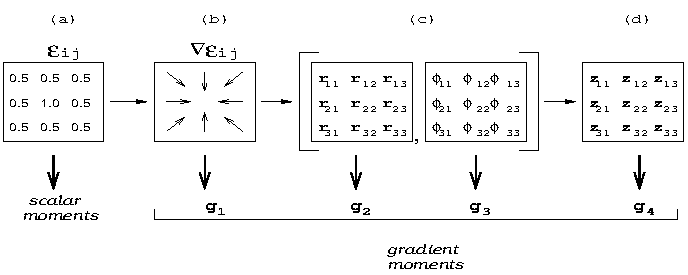
\includegraphics[width=12cm]{./figs/gpa.pdf}  
      \end{center}
      \vspace{4mm} % acrescentar o espaçamento vertical apropriado entre a borda inferior da figura e a legenda ou a fonte quando não há legenda (o valor pode ser negativo para subir)
      \legenda{Exemplo de legenda curta.} % legenda - opcional
      \label{figgpa1}
      \FONTE{\citeonline{lba/06}.} % fonte consultada (elemento obrigatório, mesmo que seja produção do próprio autor)
    \end{figure}
    \end{meucomandolf}
\end{frame}
\endgroup

\begin{frame}{Inserção de Figuras e Tabelas}
	\vspace{-1em}
    \begin{block}{Figura no Estilo do INPE}
        \begin{figure}[H]
          \begin{center}
            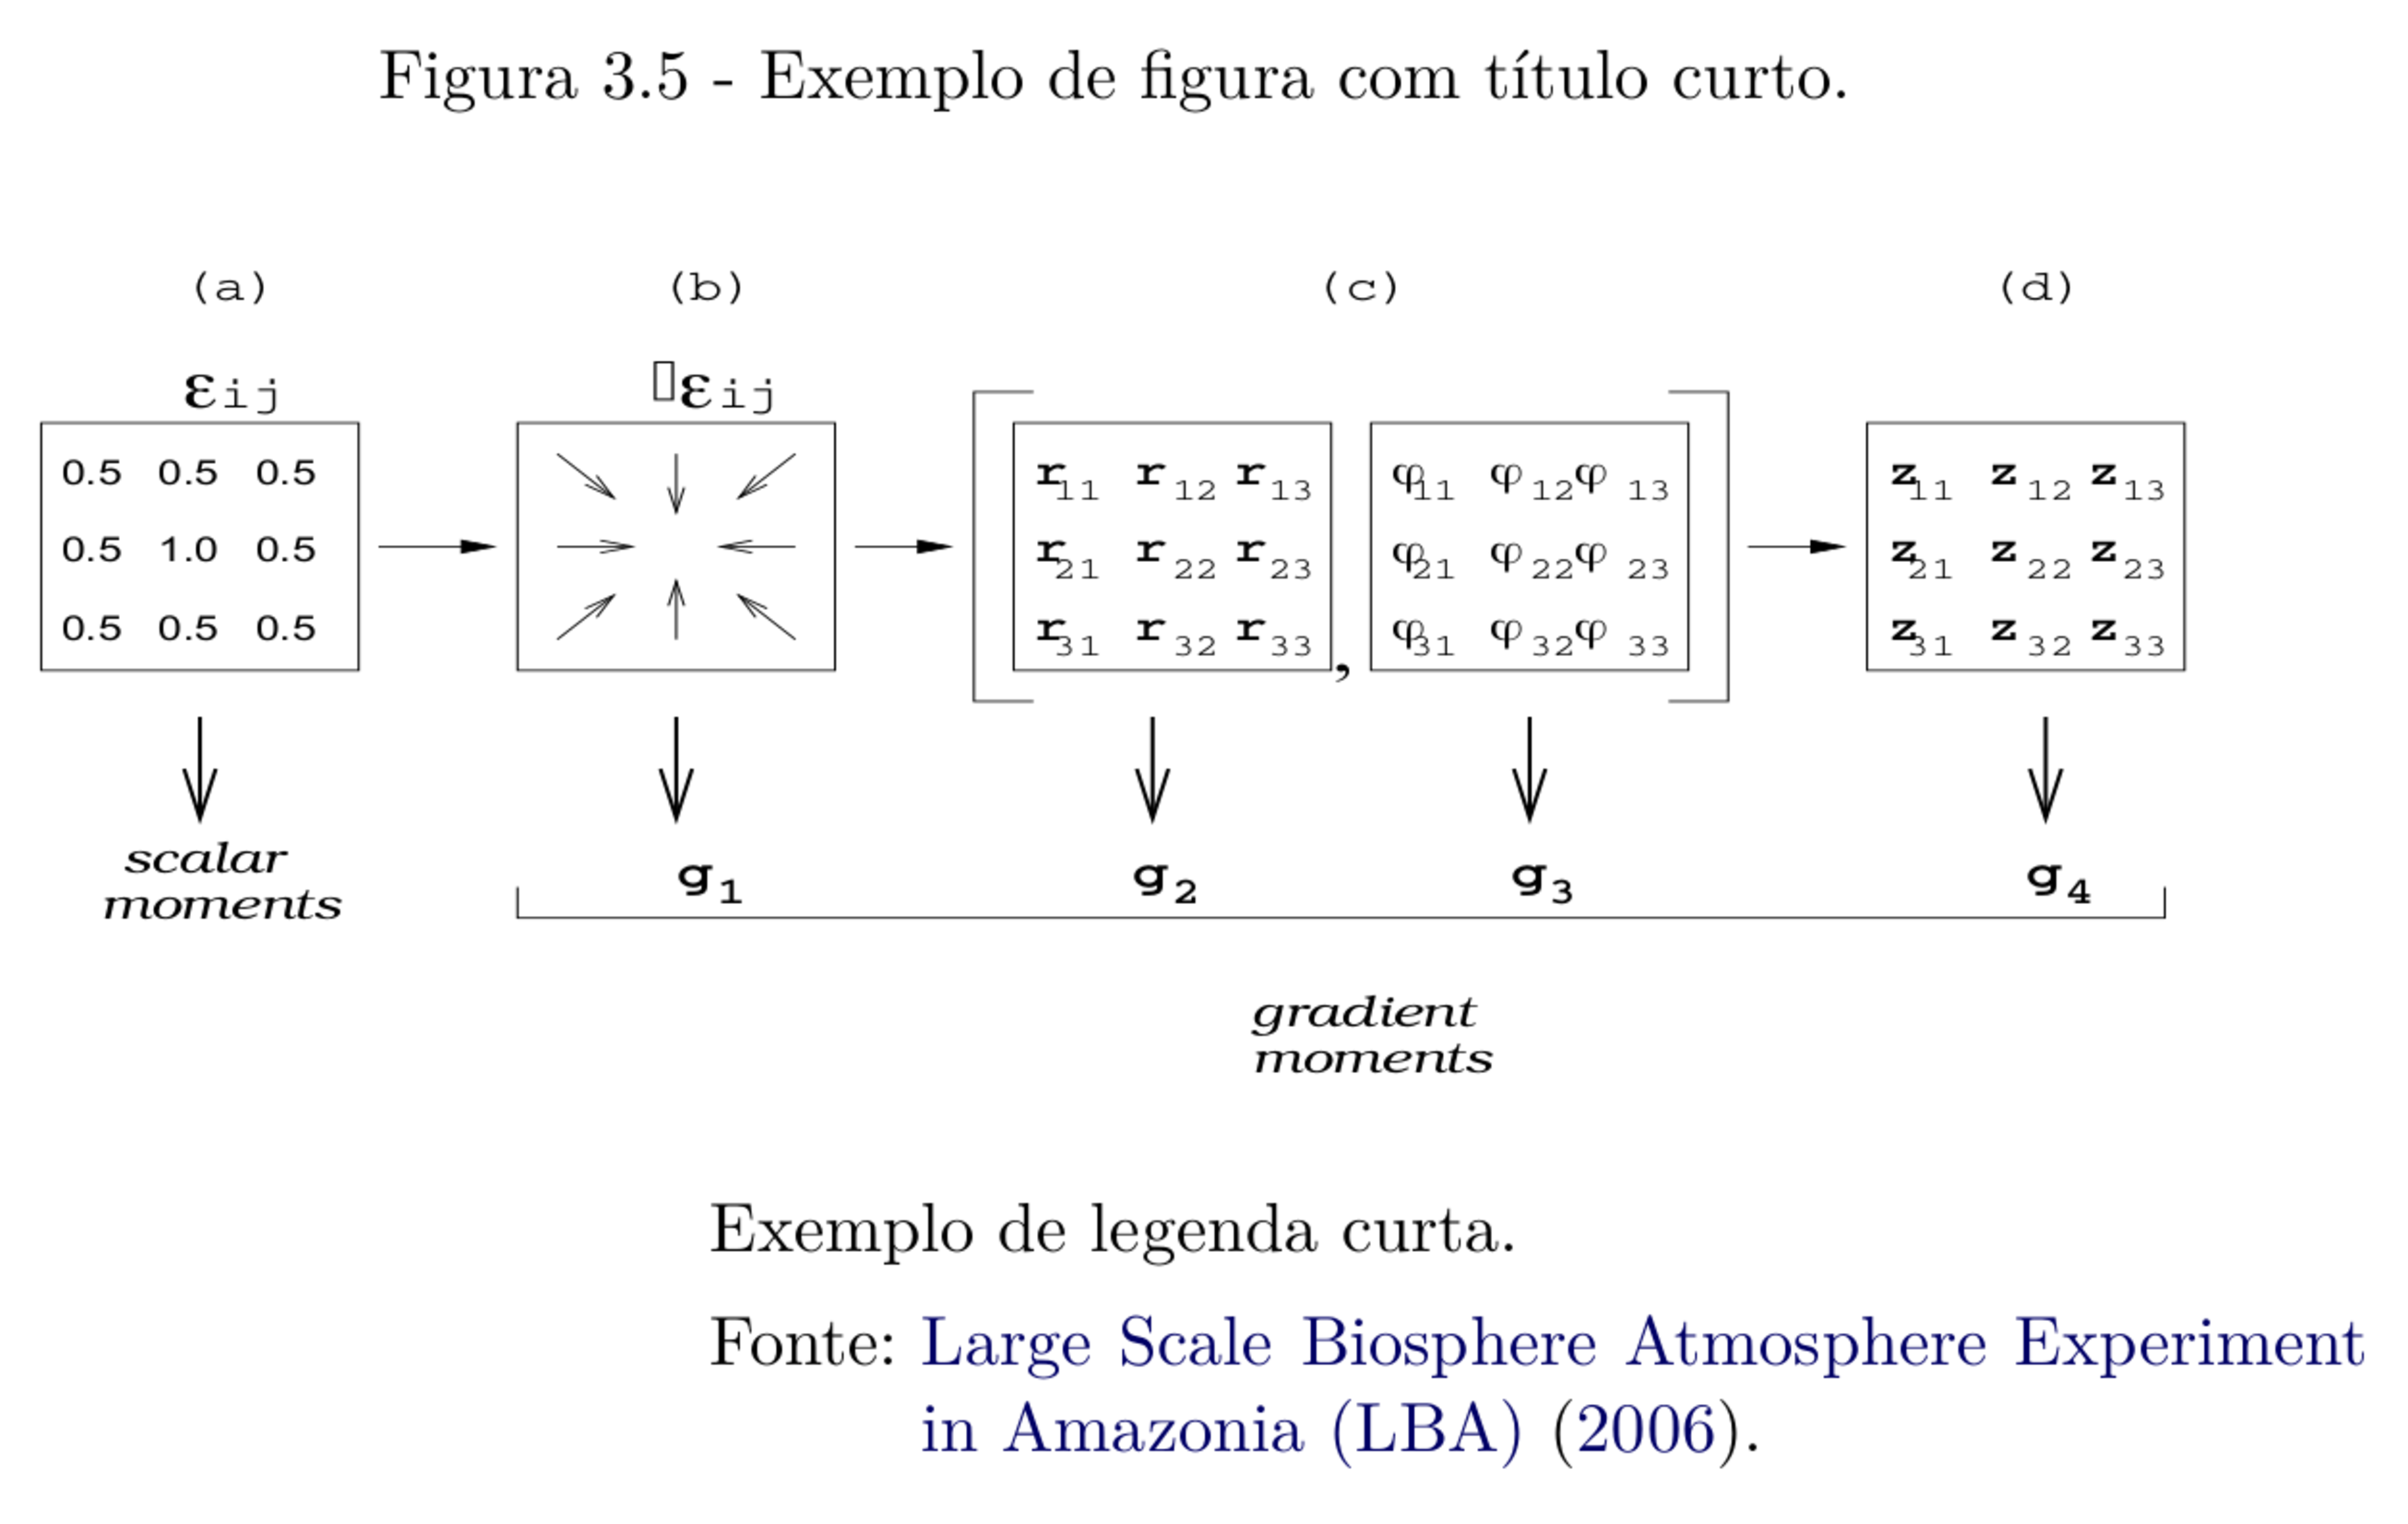
\includegraphics[width=10cm]{./figs/exefigestiinpe.pdf}  
          \end{center}
        \end{figure}
    \end{block}
\end{frame}

\begingroup
\setbeamercolor{background canvas}{bg=laranjainpe!90}
\begin{frame}[plain,fragile]{}
    \begin{meucomandolf}{Inserção de uma tabela utilizando o estilo do INPE}
        \begin{table}[H] % [htbp] opções de posicionamento da tabela no texto
            \begin{center} % use sempre um ambiente para as tabelas
            % (opções: center (recomendado), flushright, flushleft)
            % NÃO USE \centering com TABELAS se houver \FONTE!
            \caption{Exemplo de tabela, com fonte.}
            \begin{tabular}{l|l|c|c|r|r}
            \hline % desenha uma linha horizontal
            Campo 1 & Campo2 & Campo3 & Campo 4 & Campo5 & Campo6 \\
            Campo 1 & Campo2 & Campo3 & Campo 4 & Campo5 & Campo6 \\
            Campo 1 & Campo2 & Campo3 & Campo 4 & Campo5 & Campo6 \\
            \hline % desenha uma linha horizontal
            \end{tabular}
            \end{center}
            \FONTE{Coloque a fonte de referência aqui, se houver.}
        \end{table}
    \end{meucomandolf}
\end{frame}
\endgroup

\begin{frame}{Inserção de Figuras e Tabelas}
    \begin{block}{Tabela no Estilo do INPE}
        \begin{figure}[H]
          \begin{center}
            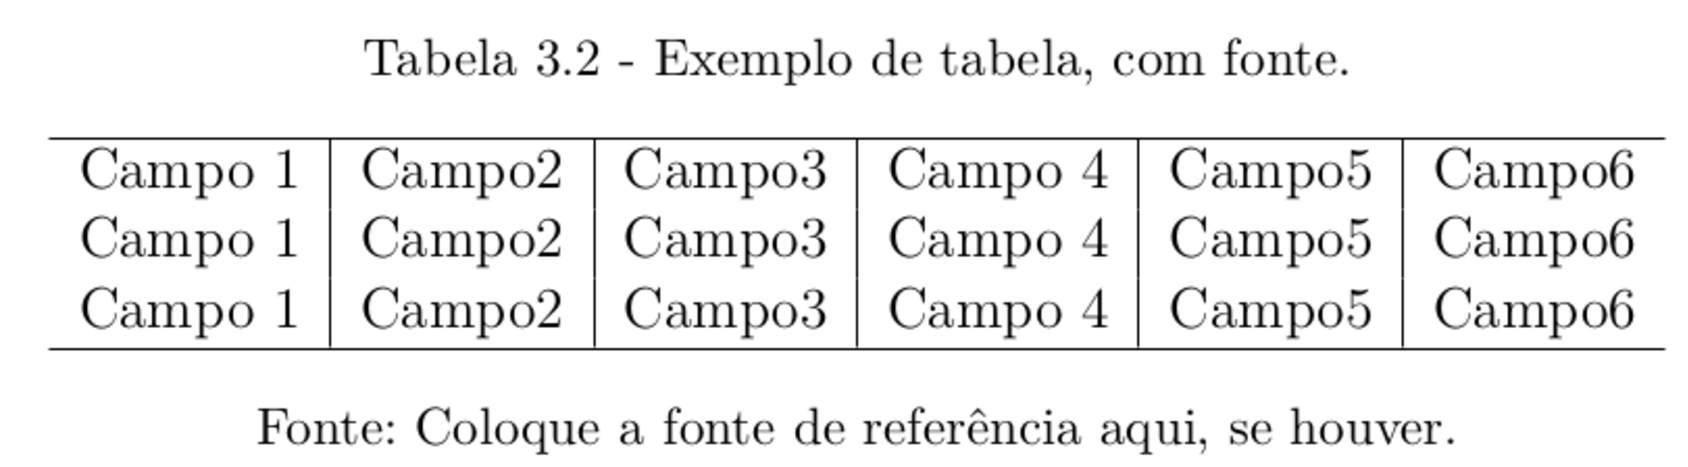
\includegraphics[width=10cm]{./figs/exetabestiinpe.pdf}  
          \end{center}
        \end{figure}
    \end{block}
\end{frame}

\begin{frame}{Inserção de Figuras e Tabelas}
    \begin{marker}
        Vários outros exemplos de figuras e tabelas podem ser encontrados em ``MANUAL PARA ELABORAÇÃO, FORMATAÇÃO E SUBMISSÃO DE TESES, DISSERTAÇÕES E OUTRAS PUBLICAÇÕES DO INPE (CEPPII, 2019)'' (\url{http://urlib.net/sid.inpe.br/iris@1916/2005/05.19.15.27}).
    \end{marker}
\end{frame}

\section{Referências}

\subsection{Inserção de Citações e Referências}

\begin{frame}{Inserção de Citações e Referências}
    \begin{block}{Formato Bib\TeX{}}
        \vspace{1em}
        \begin{itemize}
            \pause
            \item Formato específico para a organização de referências bibliográficas;
            \pause
            \item Referências ficam dentro de um arquivo de extensão {\tt .bib};
            \pause
            \item Requer cuidados especiais;
            \pause
            \item Altera a sequência de compilação.
        \end{itemize}
    \end{block}
\end{frame}

\begin{frame}{Inserção de Citações e Referências}

\tikzstyle{format} = [draw, thin, fill=blue!20]
\tikzstyle{medium} = [ellipse, draw, thin, fill=green!20, minimum height=2.5em]

\begin{figure}
\begin{tikzpicture}[node distance=3cm, auto,>=latex', thick]
    % We need to set at bounding box first. Otherwise the diagram
    % will change position for each frame.
    \path[use as bounding box] (-1,0) rectangle (9,-2);
    \path[->]<1-> node[format] (tex) {Arq. {\tt .tex}};
    \path[->]<2-> node[format, right of=tex] (dvi) {Arq. {\tt .dvi}}
                  (tex) edge node {\LaTeX} (dvi);
    %\path[->, draw]<3-> (tex) -- +(0,-1) -| node[near start] {Bib\TeX} (dvi);
    \path[->, draw=blue]<3-> (tex) -- +(0,-1) -| node[near start] {\color{blue}{Bib\TeX{}}} +(2.75,-0.3) (dvi) +(-0.25,-0.3);
    
    %\path[-> draw] (tex) -- +(0,-1) -| node[near start] (dvi + (-1,-1));
    
    \path[->, draw]<4> (-1.5,1.5) rectangle (4.5,-2) node[above right] {$\times$2};
    \path[->]<5-> node[format, right of=dvi] (ps) {Arq. {\tt .ps}}
                  node[medium, below of=dvi] (screen) {Tela}
                  (dvi) edge node {dvips} (ps)
                        edge node[swap] {xdvi} (screen);
    \path[->]<6-> node[format, right of=ps] (pdf) {Arq. {\tt .pdf}}
                  node[medium, below of=ps] (print) {Impressão}
                  (ps) edge node {ps2pdf} (pdf)
                       edge node[swap] {gs} (screen)
                       edge (print);
    \path[->]<7-> (pdf) edge (screen)
                        edge (print);
    \path[->, draw=red]<8-> (dvi) -- +(0,2) -| node[near start] {\color{red}{dvipdf}} +(6.25,0.3) (pdf);
    \path[->, draw]<9-> (tex) -- +(0,1) -| node[near start] {pdf\LaTeX} (pdf);
\end{tikzpicture}
\end{figure}
\end{frame}

\begin{frame}[fragile]{Inserção de Citações e Referências}
    \begin{block}{Compilação de um documento \LaTeX{} com referências Bib\TeX{}}
    \vspace{1em}
    \begin{meucomandot}{Compilação Manual}
            latex documento.tex
            bibtex documento
            latex documento
            latex documento
            dvips documento.dvi
            ps2pdf documento.ps
    \end{meucomandot}        
    \end{block}
\end{frame}

\begin{frame}[fragile]{Inserção de Citações e Referências}
    \begin{block}{\textit{Script} {\tt execpub.sh} do estilo do INPE (para o BASH)}
        \vspace{1em}
        \pause
        \begin{meucomandot}{Permissão para executar}
        chmod +x execpub.sh
        \end{meucomandot}
        \pause
        \begin{meucomandot}{Uso do comando}
        ./execpub.sh <arquivo> <opcao>
        \end{meucomandot}    
        \pause
        \begin{meucomandot}{Exemplo}
        ./execpub.sh publicacao pdf
        \end{meucomandot}        
    \end{block}
\end{frame}

\begin{frame}[plain,fragile]{Inserção de Citações e Referências}
	\vspace{0.5em}
    \begin{meucomandol}{Exemplo de uma referência no formato Bib\TeX{}}
        @article{fulano/1964,
            author = {Fulano, Sicrano},
             title = {Um Exemplo de Refer{\^e}ncia Bibliogr{\'a}fica do tipo article.},
           journal = {Revista Mensal de Ci{\^e}ncia},
            volume = {12},
            number = {11},
             pages = {340-346},
              year = {1964},
         }
    \end{meucomandol}
\end{frame}

\begin{frame}{Inserção de Citações e Referências}
    \vspace{-1.5em}
    \begin{table}[H]
    \centering
    \caption{Tipos de referências padrão do Bib\TeX{}.}
    \vspace{-0.5em}
    {\footnotesize
        \begin{tabular}{p{2cm}p{7.5cm}}
        \toprule
        \textbf{Tipo} & \textbf{Descrição} \\
        \midrule
        {\tt article}       & Artigo de jornal ou revista \\
        {\tt book}          & Livro publicado \\
        {\tt booklet}       & Compilação de trabalhos em formato de livro com vários autores, mas sem editora ou patrocinador \\
        {\tt inbook}        & Parte ou capítulo de um livro, sem o título do livro ao qual pertence \\
        {\tt incollection}  & Parte ou capítulo de um livro, com o título do livro ao qual pertence \\
        {\tt inproceedings} & Artigo em anais de congresso ou conferência \\
        {\tt conference}    & Idem a {\tt inproceedings} \\
        {\tt manual}        & Manual técnico \\
        {\tt masterthesis}  & Dissertação de mestrado \\
        {\tt phdthesis}     & Tese de doutorado \\
        {\tt misc}          & Modelo útil para outros tipos de referências \\
        {\tt proceedings}   & Anais de congresso ou conferência \\
        {\tt techreport}    & Relatório técnico \\
        {\tt unpublished}   & Artigo, livro ou outro tipo de trabalho não publicado \\
        \bottomrule
        \end{tabular}
    }
    \end{table}
\end{frame}

{
\setbeamertemplate{navigation symbols}{}
\setbeamertemplate{background canvas}{\includegraphics[height=\paperheight,width=\paperwidth,page=1]{refs.pdf}}
\begin{frame}[plain]
\end{frame}
}

{
\setbeamertemplate{navigation symbols}{}
\setbeamertemplate{background canvas}{\includegraphics[height=\paperheight,width=\paperwidth,page=2]{refs.pdf}}
\begin{frame}[plain]
\end{frame}
}

\begin{frame}{Para Saber Mais e Outros Recursos}
	\vspace{-1em}
	\begin{block}{Para Saber Mais}
		\begin{itemize}
			\item Apostila de Introdução ao \LaTeX (\href{https://github.com/cfbastarz/CursoIntroLaTeX}{em Português});
			\item Tutorial do \textit{Overleaf} (\href{https://pt.overleaf.com/learn/latex/}{em Inglês});
			\item StackExchange do \LaTeX (\href{https://tex.stackexchange.com/}{em Inglês});
			\item Fórum do \LaTeX{} Community (\href{https://latex.org/forum/}{em Inglês} e \href{http://latex.net.br/}{em Português}).
		\end{itemize}
	\end{block}
	\\
	\begin{block}{Outros Recursos}
		\begin{itemize}
			\item \textit{Tables Generator} (\href{https://www.tablesgenerator.com/}{em Inglês});
			\item \LaTeX{} \textit{Tables} (\href{https://www.latex-tables.com/}{em Inglês});
			\item Detexify (\href{https://detexify.kirelabs.org/classify.html}{em Inglês}).
		\end{itemize}
	\end{block}	
	\\
	\begin{block}{Repositório desta Apresentação}
		\begin{itemize}
			\item \url{https://github.com/cfbastarz/IntroLaTeXABPG}
		\end{itemize}
	\end{block}
\end{frame}

% Frame Final (NÃO MODIFICAR)
\usebackgroundtemplate%
{%
	
\includegraphics[width=\paperwidth,height=\paperheight]{./figs/fundo_slide_inpe_final.png}%
}

% Remove o rodapé no último frame
\begingroup
\setbeamertemplate{footline}{}
\begin{frame}

\end{frame}
\endgroup

\end{document}